\chapter{Analisis}

Bab ini akan membahas mengenai permasalahan umum yang dihadapi, melakukan studi kasus pada algoritma \textit{naive bayes classifier}, dan melakukan analisis pemodelan sistem yang akan dibangun.

\section{Deskripsi Masalah}
Salah satu algoritma teknik \textit{data mining} yang digunakan pada skripsi ini adalah algoritma \textit{naive bayes classifier}. Tingkat akurasi pada algoritma ini dapat dipengaruhi oleh beberapa faktor. Salah satu faktor pentingnya adalah faktor volume data. Pada algoritma \textit{naive bayes} yang diimplementasikan secara \textit{standalone}, (non-\textit{MapReduce}, tidak menggunakan komputasi secara paralel) tidak dapat mengolah proses menggunakan data yang sangat besar, karena adanya keterbatasan memori yang dimiliki oleh perangkat tersebut.

\textit{Apache hadoop} digunakan untuk menangani hal meliputi big data dengan sistem yang terdistribusi. \textit{Framework hadoop} dapat digunakan untuk membantu algoritma \textit{naive bayes classifier} dalam menangani jumlah data yang sangat banyak dengan mengesampingkan batasan memori. Rancangan program \textit{naive bayes} yang dibuat perlu berbasiskan \textit{MapReduce} pada Hadoop. Dengan begitu, tingkat akurasi yang dimiliki oleh algoritma ini akan sangat maksimal dengan memberikan fasilitas untuk mengolah data yang sangat banyak dan beragam (\textit{big data}). Waktu yang dibutuhkan untuk mengeksekusi program tersebut juga diharapkan akan sangat cepat sebanding dengan jumlah komputer/node yang digunakan pada sistem terdistribusi hadoop(mendelegasikan pekerjaan kepada tiap komputer/node yang terintegrasi pada sistem secara bersamaan). 
%Untuk dapat melakukan hal tersebut, program perlu dirancang dengan berbasis \textit{MapReduce}. Skripsi ini akan membangun perangkat lunak yang menerapkan algoritma naive bayes pada sistem terdistribusi hadoop.

\section{Kebutuhan Pemilihan Data Masukan}
Data yang dapat digunakan pada perangkat lunak yang dibuat adalah data tidak terstruktur yang menggunakan \textit{comma-separated values}\footnote{ CSV (comma-separated values) merupakan data tabular yang berada di dalam plain text. Setiap baris dari data tersebut menyatakan sebuah record. Setiap record memiliki 1 atau lebih field yang dipisahkan oleh koma}. Data tidak terstruktur (\textit{unstructured data}) adalah data yang tidak memiliki format pasti. Data tidak terstruktur biasanya merupakan data text yang berukuran sangat besar dan format dari isi datanya juga dapat memiliki format yang bermacam - macam, seperti: tanggal ; angka ; suatu kejadian ; dsb. 
Data - data yang digunakan bisa saja berupa data pencatatan pembelian selama 3 tahun terakhir dari suatu perusahaan, data penjualan mobil dengan spesifikasi kriteria yang rinci dari suatu perusahaan mobil, dsb. Selain itu, data yang digunakan juga perlu memiliki ukuran yang cukup besar (supaya manfaat dari penggunaan framework hadoop akan lebih terlihat signifikan). Seperti pada contoh data berikut mengenai penentuan seseorang akan bermain tenis atau tidak jika diberikan beberapa fakta yang terjadi terkait faktor lingkungan dan waktu :

\begin{lstlisting}
Outlook,Temperature,Humidity,Windy,Play,Rand,Hour
Rainy,Hot,High,FALSE,No,3.5,12:00:00
Rainy,Hot,High,TRUE,No,12,14:00:00
Overcast,Hot,High,FALSE,Yes,11,,16:00:00
Sunny,Mild,High,FALSE,Yes,4,,18:00:00
Sunny,Cool,Normal,FALSE,Yes,2,09:00:00
Sunny,Cool,Normal,TRUE,No,1.9,17:00:00
Overcast,Cool,Normal,TRUE,Yes,6.4,20:00:00
Rainy,Mild,High,FALSE,No,10,07:00:00
Rainy,Cool,Normal,FALSE,Yes,9,06:00:00
\end{lstlisting}
Pada kolom pertama, ke-dua, ke-tiga, ke-empat, dan ke-lima merupakan data yang bertipe diskrit dan pada kolom ke-enam dan ke-tujuh merupakan data yang bertipe numerik. Tetapi, pada kolom ke-tujuh, perlu diberikan penanganan lebih lanjut karena data tersebut perlu dikonversi terlebih dahulu dari yang berbentuk jam ke bentuk numerik yang sederhana.

\section{Kebutuhan Pra-pengolahan Data}

Pada teknik data mining, diperlukan fase pra-pengolahan data terlebih dahulu sebelum melakukan mining dengan teknik tertentu, agar data yang masuk ke dalam perangkat lunak memiliki format yang pasti. Pada skripsi kali ini, fase pra-pengolahan akan diperlukan untuk mendeteksi dan menangani terjadinya \textit{missing values}\footnote{\textit{Missing-values} merupakan keadaan dimana jumlah field pada suatu record tidak memenuhi jumlah field yang seharusnya} pada data. Pendekatan yang digunakan untuk mengatasi terjadinya \textit{missing-values} yang dapat menyebabkan analisis berjalan tidak lancar ini adalah metode \textit{listwise deletion}. \textit{Listwise deletion} merupakan salah satu metode dalam cabang ilmu statistika untuk mengatasi terjadi \textit{missing-values} dengan cara mengabaikan seluruh record - record yang memiliki \textit{missing-values} \cite{PeughMissing:2004}.

\begin{figure}[ht]
	\centering
	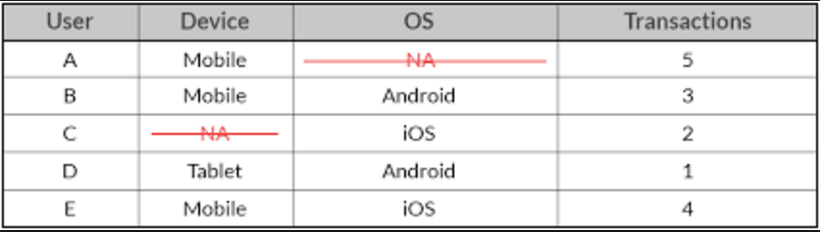
\includegraphics[scale=0.5]{GambarIO/Missing-values}
	\caption[Missing-values]{Missing-values \cite{MissingVal:2016}} 
	\label{fig:Missing-values}
\end{figure}

\section{Perhitungan Manual Dengan Data Studi Kasus}

\subsection{Studi kasus pembuatan model \textit{naive bayes classifier}}
%\subsubsection{Tahapan Membuat Model Klasifikasi Dari Algoritma Naive Bayes}		
Misal kita memiliki dataset yang menunjukan seseorang akan bermain tenis atau tidak berdasarkan dari data kelembaban dan pemandangan yang terjadi seperti pada tabel \ref{tab:dataset} berikut: 
		
		\begin{table}[H]
		\label{tab:dataset}
		\centering
		\caption{Contoh Dataset (atribut kelas = \textbf{Play})}
		\begin{tabular}{ | c | c | c | }
		\hline
		%\toprule
		 Humidity & Outlook & \textbf{Play}\\ \hline \hline
		%\midrule
		60 & Rainy & No\\ \hline
		%\midrule
		78 & Rainy & No\\ \hline
		%\midrule
		80 & Sunny & Yes\\ \hline
		%\midrule
		75 & Sunny & No\\ \hline
		%\midrule
		85 & Sunny & Yes \\ \hline
		%\bottomrule
		\end{tabular}
		\end{table}
		
		
		Langkah pertama yang perlu dilakukan untuk membuat algoritma naive bayes classifier adalah membuat table frekuensi untuk setiap atribut prediktor terhadap atribut kelas yang bertipe Diskrit. Pada contoh tabel diatas, diasumsikan bahwa atribut Humidity dan Outlook merupakan atribut prediktor, lalu untuk atribut Play merupakan atribut kelas.
		
		\begin{table}[ht]
			\centering
			\caption{Table frekuensi atribut Outlook}
			\begin{tabular}{ | c | c | c | c | }
			\hline
			 & \multicolumn{2}{c}{\textbf{Play}} & \\ 
			%\hline
			 & Yes & No & \textit{sum} \\
			\hline
			Sunny & 2 & 1 & \textbf{3}\\
			\hline
			Rainy & 0 & 2 & \textbf{2} \\
			\hline
			\textit{sum} & \textbf{2} & \textbf{3} & \\
			\hline
			\end{tabular}
		\end{table}
		
		Pada table frekuensi untuk atribut Outlook, dapat dilihat bahwa $P(X=Rainy|C=Yes) = 0$. Naive bayes classifier tidak dapat mengatasi frekuensi yang nilainya 0. Karena dapat menyebabkan seluruh perhitungan menjadi 0(karena berapapun bilangannya, jika dikalikan dengan 0 akan selalu menghasilkan nilai 0), sehingga menjadi tidak relevan. Pendekatan yang perlu digunakan untuk mengatasi hal tersebut adalah dengan menggunakan metode Laplacian Correction (->Pustaka.Bib). Pada metode tersebut, dikatakan bahwa kita perlu menambah nilai 1 kepada seluruh nilai pada table frekuensi untuk mengatasi masalah \textit{zero-frequency problems}. Asumsikan training database (D) itu sangat besar, dimana menambahkan frekuensi sebanyak 1 ke setiap jumlah perhitungan yang kita perlukan tidak akan memberikan pengaruh yang besar terhadap nilai kemungkinan akhir (Laplacian correction / Laplace estimator) \cite{PeughMissing:2004}. Perubahan nilai atribut dapat dilihat pada table 3. \\
		
		\begin{table}[ht]
			\centering
			\caption{Table frekuensi atribut Outlook}
			\begin{tabular}{|c|c|c|c|}
			\hline
			 & \multicolumn{2}{c}{\textbf{Play}} & \\
			 & Yes & No & \textit{sum} \\ 
			\hline
			Sunny & 3 & 2 & \textbf{5}\\
			\hline
			Rainy & 1 & 3 & \textbf{4} \\
			\hline
			\textit{sum} & \textbf{4} & \textbf{5} & \\
			\hline
			\end{tabular}
		\end{table}
		
		
		Langkah kedua adalah membuat table kemungkinan dari table frekuensi yang telah dibuat :		
		\begin{table}[ht]
			\centering
			\caption{Table kemungkinan atribut Outlook}
			\begin{tabular}{|c|c|c|c|}
			\toprule
			 & \multicolumn{2}{c}{\textbf{Play}} & \\
			 & Yes & No & \textit{sum} \\ 
			\midrule
			Sunny & 3/4 & 2/5 & \textbf{5/9}\\
			\midrule
			Rainy & 1/4 & 3/5 & \textbf{4/9} \\
			\midrule
			\textit{sum} & \textbf{4/9} & \textbf{5/9} & \\
			\bottomrule
			\end{tabular}
		\end{table}
		
		Karena atribut Humidity bertipe numerik, atribut tersebut perlu diubah ke dalam kategori mereka masing - masing agar perhitungan dalam pembuatan model dapat tepat. Konversi atribut yang bertipe numerik bisa menggunakan distribusi variabel numerik untuk dapat menebak frekuensi-nya dengan mengasumsikan distribusi normal untuk variabel numerik. Rumus yang digunakan adalah :\\
		
		\textbf{Mencari mean (rata - rata)} 
		\begin{equation}
			\mu = \dfrac{1}{n} \mathlarger{\mathlarger{‎‎\sum}}_{i=1}^{n‎}x_i‎‎
		\end{equation}
		
		\textbf{Mencari Standard Deviation}
		\begin{equation}
			\sigma = \mathlarger{[ \dfrac{1}{n - 1} \mathlarger{\mathlarger{‎‎\sum}}_{i=1}^{n‎} (x_i‎‎ - \mu)^2]}^{0.5}
		\end{equation}
		
		\textbf{Normal Distribution}
		\begin{equation}
			f(x) = \dfrac{1}{\sqrt{2\pi\sigma}}e^{-\dfrac{(x-\mu)^2}{2\sigma^2}}
		\end{equation}
		
		Berikut merupakan table rata - rata dan standar deviasi dari atribut Humidity yang bertipe numerik : 
		
		\begin{table}[h]
		\centering
		\caption{Table rata - rata dan standar deviasi atribut Humidity}
		\begin{tabular}{|c|c|c|c|c|}
		\toprule
		\multirow{2}{*}{Play Golf ?} & Yes & 80 & 85 & \\
		 & No & 60 & 75 & 78 \\
		\bottomrule
		\end{tabular}
		\end{table}
		
		\begin{table}[ht]
		\centering
		\caption{Table Distribusi}
		\begin{tabular}{|c|c|c|}
		\toprule
		 & Mean & StDev \\
		Yes & 82.5 & 3.5 \\
		No & 71 & 9.6 \\
		\bottomrule
		\end{tabular}
		\end{table}
		
		Dari table distribusi tersebut didapatkan formula untuk menghitung klasifikasi untuk atribut Humidity adalah:
		
		\begin{equation}
			%f(x|play=yes) = \dfrac{1}{\sqrt{2\pi(3.5)}}e^{-\dfrac{(x-82.5)^2}{2(3.5)^2}} 
			f(x|play=yes) = \dfrac{1}{\sqrt{2\pi(3.5)}}e^{-\dfrac{(x-82.5)^2}{2(3.5)^2}}
		\end{equation}
		\begin{equation}
			f(x|play=no) = \dfrac{1}{\sqrt{2\pi(9.6)}}e^{-\dfrac{(x-71)^2}{2(9.6)^2}} 
		\end{equation}
		
		\textit{Cara ini dapat diberlakukan juga pada atribut yang bertipe kontinu.}
		
		Setelah semua model dari naive bayes classifier telah jadi, maka klasifikasi sudah dapat dilakukan dengan model diatas.

\subsection{Studi kasus melakukan klasifkasi menggunakan model \textit{naive bayes classifier} yang telah dibuat sebelumnya}
%\subsection{Contoh perhitungan klasifikasi algoritma naive bayes}		
		Dimisalkan kita memiliki 2 buah dataset yang akan diuji menggunakan model klasifikasi yang telah dibangun sebelumnya, seperti berikut :
		
\begin{enumerate}
	\item $X = {Humidity = 50, Outlook = Sunny}$
	\item $Y = {Humidity = 90, Outlook = Sunny}$
\end{enumerate}
		
Untuk dataset X dan Y, akan dicari peluang kelas yang paling tinggi. \\
		
$( C_{MAP} = \underset{c \in C}{ argmax } P(c|d) = \underset{c \in C}{ argmax } \dfrac{P(d|c) P(c)}{P(d)} = \underset{c \in C}{ argmax } P(d|c) P(c) )$
		
\paragraph{Untuk dataset X dengan $P=Yes$:}
	Menghitung peluang untuk atribut $Outlook=Sunny$ dengan $P=Yes$
	\begin{displaymath}
			P(Outlook=Sunny|Yes) = 3/4 
			= 0.75
	\end{displaymath}
	
	Menghitung peluang untuk atribut $Humidity=50$ dengan $P=Yes$
		\begin{displaymath}
			P(Humidity=50|Yes) 
			= \dfrac{1}{\sqrt{2\pi(3.5)}}e^{-\dfrac{(\textbf{50}-82.5)^2}{2(3.5)^2}}
			= 4.031
		\end{displaymath}
	
	\paragraph{Untuk dataset X dengan $P=No$:}
		Menghitung peluang untuk atribut $Outlook=Sunny$ dengan $P=No$
		\begin{displaymath}
			P(Outlook=Sunny|No) = 2/5 
			= 0.4
		\end{displaymath}
		Menghitung peluang untuk atribut $Humidity=50$ dengan $P=No$
		\begin{displaymath}
			P(Humidity=50|No) 
			= \dfrac{1}{\sqrt{2\pi(9.6)}}e^{-\dfrac{(\textbf{50}-71)^2}{2(9.6)^2}}
			= 0.011
		\end{displaymath}
	\paragraph{Kesimpulan untuk $dataset$ $X$}
	Dari perhitungan di atas, didapat bahwa : \\ \\
	Untuk kelas $Play=Yes$ \\
	$P(Play=Yes|X) \\
	= P(Outlook=Sunny|Play=Yes)*P(Humidity=50|Play=Yes)*P(Yes) \\
	= 0.75 * 4.031 * 4/9 \\
	= 1.343$ \\ \\
	Untuk kelas $Play=No$ \\
	$P(Play=No|X) \\
	= P(Outlook=Sunny|Play=No)*P(Humidity=50|Play=No)*P(No) \\
	= 0.4 * 0.011 * 5/9 \\
	= 0.002$ \\ \\
	Setelah itu, lakukan normalisasi terhadap nilai - nilai berikut: \\
	$P(Play=Yes|X) = 1.343 / (1.343+0.002) \\
	= 0.998 (99.8\%)$ \\
	$P(Play=No|X) = 0.002 / (1.343+0.002) \\
	= 0.002 (0.2\%)$ \\
	
	Karena, $P(Play=Yes|X) > P(Play=No|X)$, maka hasil klasifikasi untuk \textit{dataset X} ialah kelas $Play=Yes$.
	
	\paragraph{Untuk dataset Y dengan $P=Yes$:}
	Menghitung peluang untuk atribut $Outlook=Sunny$ dengan $P=Yes$
	\begin{displaymath}
			P(Outlook=Sunny|Yes) = 3/4 
			= 0.75
	\end{displaymath}
	
	Menghitung peluang untuk atribut $Humidity=90$ dengan $P=Yes$
		\begin{displaymath}
			P(Humidity=90|Yes) 
			= \dfrac{1}{\sqrt{2\pi(3.5)}}e^{-\dfrac{(\textbf{90}-82.5)^2}{2(3.5)^2}}
			= 0.021
		\end{displaymath}
	
	\paragraph{Untuk dataset Y dengan $P=No$:}
	Menghitung peluang untuk atribut $Outlook=Sunny$ dengan $P=No$
	\begin{displaymath}
				P(Outlook=Sunny|No)
				= 2/5 
				= 0.4
		\end{displaymath}
	
	Menghitung peluang untuk atribut $Humidity=90$ dengan $P=No$
		\begin{displaymath}
			P(Humidity=90|No)
			= \dfrac{1}{\sqrt{2\pi(9.6)}}e^{-\dfrac{(\textbf{90}-71)^2}{2(9.6)^2}} 
			= 0.018
		\end{displaymath}
		
	\paragraph{Kesimpulan untuk $dataset$ $Y$}
	Dari perhitungan di atas, didapat bahwa : \\ \\
	Untuk kelas $Play=Yes$ \\
	$P(Play=Yes|Y) \\
	= P(Outlook=Sunny|Play=Yes)*P(Humidity=90|Play=Yes)*P(Yes) \\
	= 0.75 * 0.021 * 4/9 \\
	= 0.007$ \\ \\
	Untuk kelas $Play=No$ \\
	$P(Play=No|Y) \\
	= P(Outlook=Sunny|Play=No)*P(Humidity=90|Play=No)*P(No) \\
	= 0.4 * 0.018 * 5/9 \\
	= 0.004$ \\ \\
	Setelah itu, lakukan normalisasi terhadap nilai - nilai berikut: \\
	$P(Play=Yes|Y) = 0.007 / (0.007+0.004) \\
	= 0.64 (64\%)$ \\
	$P(Play=No|Y) = 0.004 / (0.007+0.004) \\
	= 0.46 (46\%)$ \\
	
	Karena, $P(Play=Yes|Y) > P(Play=No|Y)$, maka hasil klasifikasi untuk \textit{dataset Y} ialah kelas $Play=Yes$.
	

\section{Analisis Perangkat Lunak}

	Pada bagian ini akan dijelaskan menenai analisis perancangan perangkat lunak yang mencakup aliran proses dan gambaran secara umum diagram kelas untuk melakukan skema algoritma \textit{naive bayes classifier} berbasis \textit{map reduce}.

\subsection{Analisis Skema Algoritma \textit{Naive Bayes Classifier} Berbasis \textit{Map Reduce}}

\begin{figure}[ht]
	\centering
	\includegraphics[scale=0.65]{GambarIO/Rancangan-NB-M-R}
	\caption[Rancangan Keseluruhan Modul Program]{Rancangan Keseluruhan Modul Program}
	\label{fig:Rancangan Keseluruhan Modul Program}
\end{figure}

%Perangkat lunak yang dibangun akan mem
Keseluruhan program yang akan menjalankan pelatihan maupun pengujian klasifikasi naive bayes berbasis mapreduce pada Hadoop yang dibuat akan memiliki 4 buah modul. sebagian besar modul tersebut harus berjalan secara berurutan dan saling bergantung satu dengan lainnya dalam menjalankan tugasnya. Berikut adalah spesifikasi ringkas dari modul beserta urutan yang perlu dijalankan terlebih dahulu: 

\begin{figure}[H]
	\centering
	\includegraphics[scale=0.65]{GambarIO/Modul-Specification}
	\caption[Modul-Specification]{Modul Specification}
	\label{fig:Modul Specification}
\end{figure}

\subsubsection{Modul Kelola \textit{Input}}

Pada Modul Input, program akan menerima input file dari pengguna berupa data yang akan dijadikan pelatihan untuk pembuatan model klasifikasi naive bayes. Pengguna diberikan pilihan untuk menentukan atribut mana saja yang akan dijadikan kelas dan yang dijadikan sebagai atribut prediktor dan memilih tipe konten dari atribut yang digunakan (mis: \textit{diskrit atau numerik}). Selain itu, penguna juga diberikan pilihan untuk membagi presentase seluruh data input yang akan dijadikan sebagai \textit{data training} dan \textit{data testing}. Program pada modul ini akan meminta akses kepada server master Hadoop untuk melakukan proses tulis pada HDFS dengan meng-import library Hadoop Client API pada program. Pada modul ini terdapat file tambahan yang akan dimasukan ke dalam HDFS, yaitu file yang bernama meta.info. File meta.info ini akan berisi kumpulan dari atribut prediktor yang pengguna pilih dan atribut kelas yang penggna pilih beserta dengan masing - masing tipe kontennya.

Berikut merupakan diagram \textit{flow chart} untuk modul input:

\begin{figure}[H]
	\centering
	\label{fig:flow_input}
	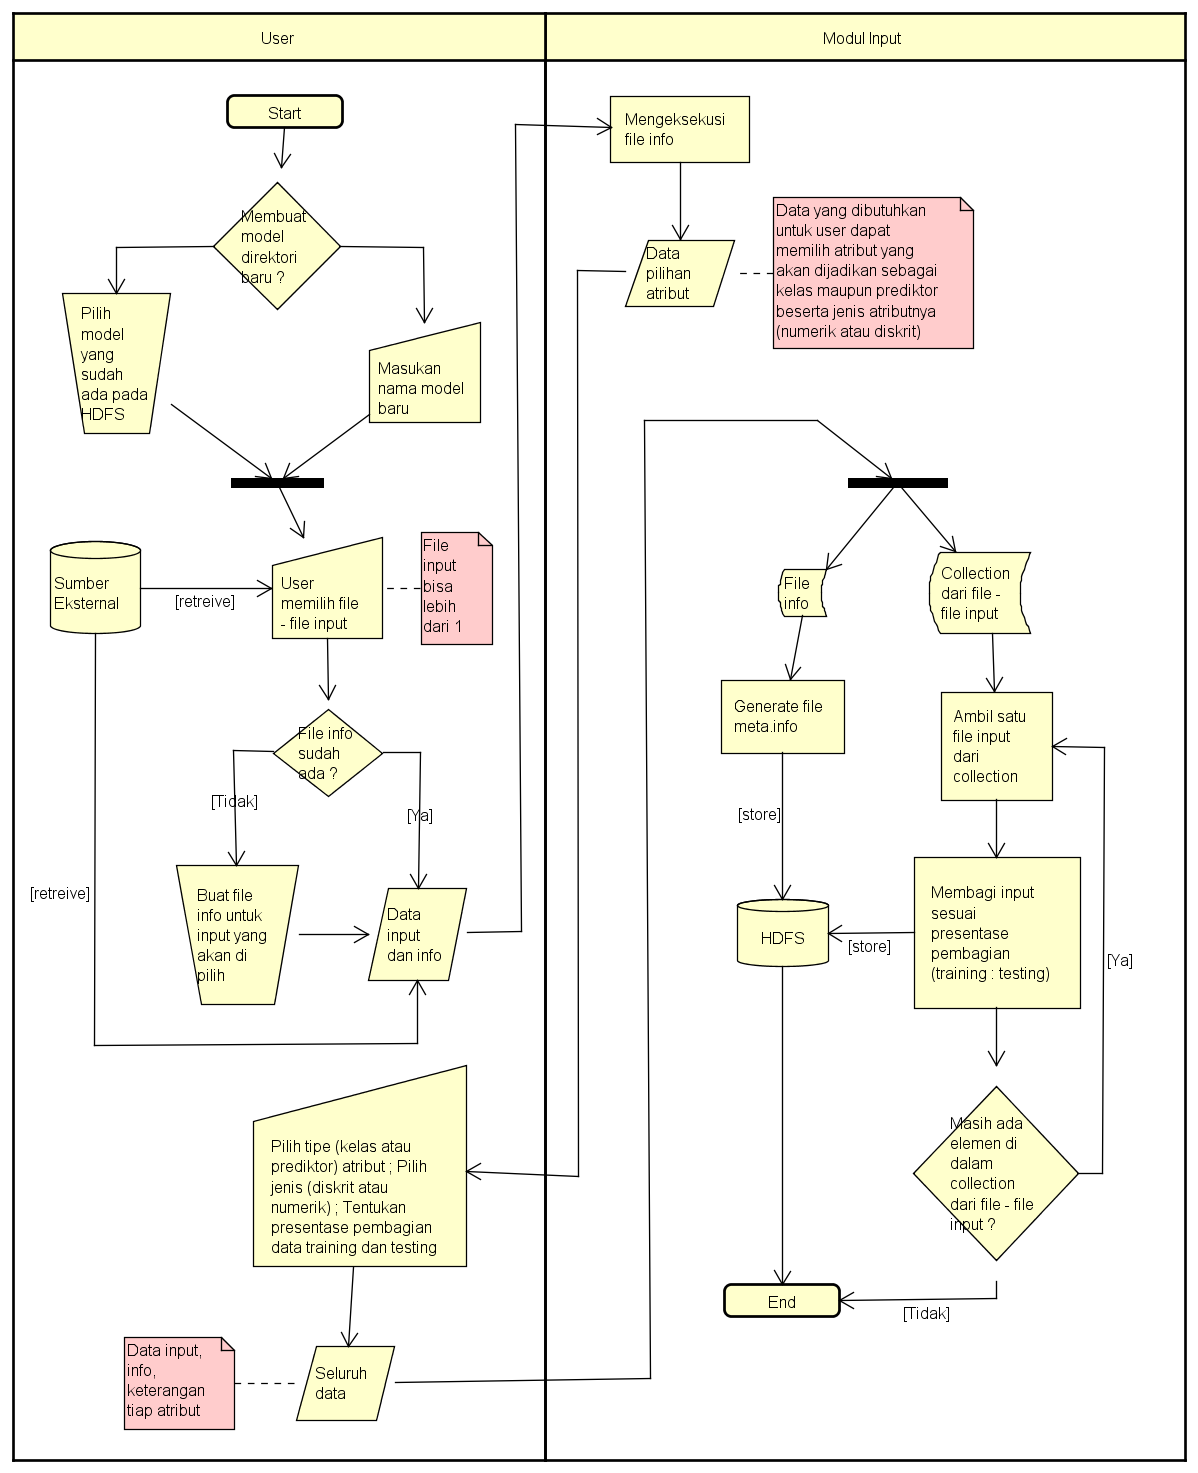
\includegraphics[scale=0.55]{Diagram/Flowchart_Input}
	\caption[Flow Chart Modul Input]{Flow Chart Modul Input}
	\label{fig:Flow Chart Modul Input}
\end{figure}

\subsubsection{Modul \textit{Train Naive Bayes M-R Based}}

Sebelum modul ini dijalankan, proses pada modul Input haruslah terlebih dulu selesai, karena file yang menjadi input pada modul ini merupakan hasil dari salinan file yang dijalankan pada proses dalam modul Input. Pada modul ini akan dijalankan proses train dalam pembentukan model klasifikasi naive bayes. Program \textit{training} klasifikasi naive bayes dibuat di atas framework mapreduce yang akan dijalankan pada Hadoop. Terdapat 2 pengecekan yang akan dilakukan pada modul ini, yaitu untuk menghitung atribut yang bertipe diskrit dan numerik(kontinu).\\
	Program pada modul ini akan memisahkan cara perhitungan yang digunakan dalam membangun sebuah model \textit{naive bayes classifier}. Algoritma Naive Bayes yang akan diimplementasikan pada program akan menerima input berupa dataset dan info mengenai dataset tersebut. Info yang akan diberikan meliputi atribut yang digunakan untuk melakukan pembuatan model classifier, tipe dari tiap atribut yang akan digunakan, dan atribut yang akan menjadi kelas-nya.
	
Berikut merupakan diagram \textit{flow chart} untuk modul \textit{training}:

\begin{figure}[H]
	\centering
	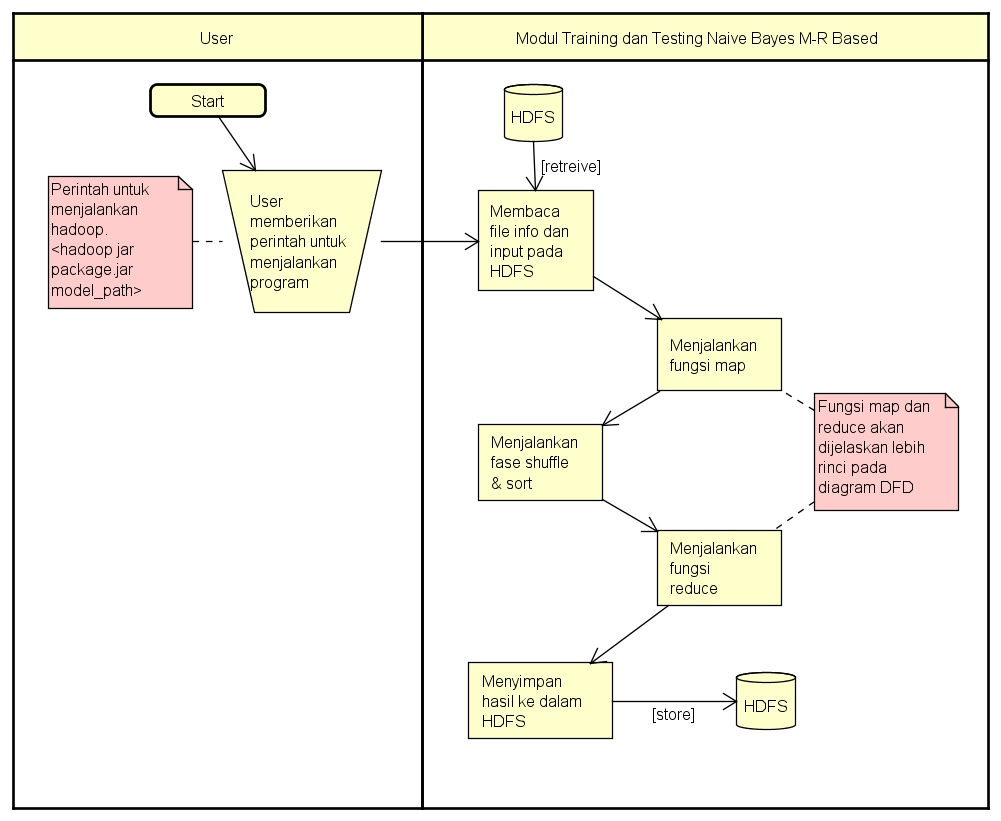
\includegraphics[scale=0.65]{Diagram/Flowchart_Training_Testing_MR}
	\caption[Flow Chart Modul Training]{Flow Chart Modul Training}
	\label{fig:Flow Chart Modul Training}
\end{figure}

Untuk proses yang berbasis \textit{MapReduce} pada modul ini perlu digambarkan menggunakan DFD, agar bisa tergambarkan lebih rinci mengenai detail proses tersebut. Berikut merupakan \textit{context diagram}\footnote{\textit{Context Diagram biasa disebut juga sebagai DFD level 0.}} dan DFD untuk proses \textit{MapReduce} pada modul \textit{training}:

\paragraph{\textit{Context Diagram} Modul \textit{Training}}
\begin{figure}[H]
	\label{DFD_0_Training}
	\centering
	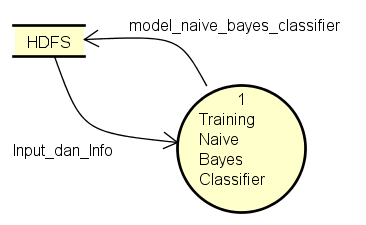
\includegraphics[scale=0.65]{Diagram/DFD_0_Training}
	\caption[\textit{Context diagram} modul Training]{\textit{Context diagram} modul Training}
	\label{fig:Context diagram modul Training}
\end{figure}

\paragraph{\textit{Data Dictionary} \textit{Context Diagram} Modul \textit{Training}}
\begin{enumerate}
	\item{Data \verb|model_naive_bayes_classifier|}
	\begin{itemize}
		\item \textit{Class Name} = [A..Z|a..z] \textcolor{red}{*}\textit{required}
		\item \textit{Class Value} = [A..Z|a..z] \textcolor{red}{*}\textit{required}
		\item \textit{Atribute Type} = [A..Z|a..z] \textcolor{red}{*}\textit{required}
		\item Frekuensi kemunculan = [0..9] \textcolor{red}{*}\textit{required}
		\item \textit{Predictor Name} = [A..Z|a..z]
		\item \textit{Predictor Value} = [A..Z|a..z]
		\item \textit{Mean} = [0..9]
		\item \textit{Sigma (standard deviation)} = [0..9]
	\end{itemize}
	Contoh data \verb|model_naive_bayes_classifier|:
	\begin{lstlisting}
	Play,Yes,2.0|CLASS
	Play,No,3.0|CLASS
	Humidity,Play,Yes ;82.5|3.5|NUMERIC
	Humidity,Play,No ;71.0|9.6|NUMERIC
	Outlook,Sunny,Play,Yes,2.0|DISCRETE
	Outlook,Sunny,Play,No,1.0|DISCRETE
	Outlook,Rainy,Play,No,2.0|DISCRETE
	\end{lstlisting}
		
	\item{Data \verb|input_dan_info|}
	\begin{itemize}
		\item Data nilai tiap field = [A..Z|a..z|0..9] \textcolor{red}{*}\textit{required}
		\item Nama - nama field = [A..Z|a..z] \textcolor{red}{*}\textit{required}
	\end{itemize}
	Contoh data \verb|input_dan_info|:
	\begin{lstlisting}
	<- Data input ->	
	Sunny,Mild,Normal,FALSE,Yes,5
	Rainy,Mild,Normal,TRUE,Yes,4.5
	Overcast,Mild,High,TRUE,Yes,3.1
	Overcast,Hot,Normal,FALSE,Yes,8.2
	Sunny,Mild,High,TRUE,No,3
	<- Data info ->
	Outlook,Temperature,Humidity,Windy,Rand
	\end{lstlisting}
\end{enumerate}


\paragraph{DFD \textit{level} 1}
\begin{figure}[H]
	\centering
	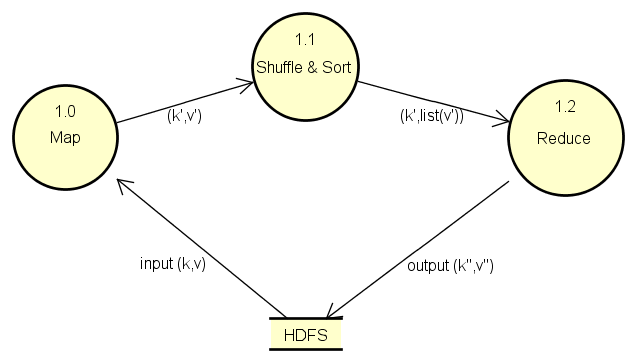
\includegraphics[scale=0.65]{Diagram/DFD_1_0_Training_Testing}
	\caption[DFD level 0 modul Training]{DFD level 0 modul Training}
	\label{fig:DFD level 0 modul Training}
\end{figure}

\paragraph{\textit{Data Dictionary} pada DFD \textit{level} 1}
\begin{enumerate}
	\item{Data \verb|input(k,v)|}
		\begin{itemize}
			\item Key: \textit{NULL}. Karena, memang pada pertama kali data diambil dari HDFS, key-nya belum terdefinisi.
			\item Value: Nilai dari tiap field yang ada = [A..Z|a..z|0..9] \textcolor{red}{*}\textit{required}
		\end{itemize}
		Contoh data \verb|input_dan_info|:
		\begin{lstlisting}
		key		value		
				Sunny,Mild,Normal,FALSE,Yes,5
				Rainy,Mild,Normal,TRUE,Yes,4.5
				Overcast,Mild,High,TRUE,Yes,3.1
				Overcast,Hot,Normal,FALSE,Yes,8.2
				Sunny,Mild,High,TRUE,No,3
		\end{lstlisting}
	\item{Data \verb|(k',v')|}
		\begin{itemize}
			\item \textit{Key} terdiri dari:
			\begin{enumerate}
				\item \textit{Class Name} = [A..Z|a..z] \textcolor{red}{*}\textit{required}
				\item \textit{Class Value} = [A..Z|a..z] \textcolor{red}{*}\textit{required}
				\item \textit{Attribute Type} = [A..Z|a..z] \textcolor{red}{*}\textit{required}
				\item \textit{Predictor Name} = [A..Z|a..z]
				\item \textit{Predictor Value} = [A..Z|a..z|0..9]
			\end{enumerate}
			\item \textit{Value} memiliki 3 jenis format yang berbeda untuk tiap jenis atribut, diantaranya adalah: 
			\begin{enumerate}
				\item Nilai dari atribut numerik dan \textit{kelas} = [0..9]
				\item Diskrit: Frekuensi kemunculan = [1] (frekuensi kemunculan untuk satu probabiltas posterior pasti bernilai 1)
			\end{enumerate}
		\end{itemize}
			Contoh data \verb|(k',v')|:
			\begin{lstlisting}
			key									value		
			|_class|Play,Yes					1
			|disc|Humidity,High,Play,No			1
			|cont|Rand,Play,Yes					34.2
			\end{lstlisting}

	\item{Data \verb|(k',list(v'))|}
	\begin{itemize}
		\item Format data untuk variabel \textit{key}, masih sama dengan format variabel \textit{key} pada data \verb|(k,v)|.
		\item Untuk variabel \textit{value} juga demikian, tetapi tipe-nya berubah menjadi list.
	\end{itemize}
	Contoh data \verb|(k',list(v'))|
	\begin{lstlisting}
		key										list_of_value		
			|_class|Play,Yes					[1,1,1,1]
			|disc|Humidity,High,Play,No			[1,1]
			|cont|Rand,Play,Yes					[34.2,23.3,15.0]
	\end{lstlisting}
	\item{Data \verb|input(k",v")|}
	\begin{itemize}
		\item Format data untuk variabel \textit{key}, sama dengan format variabel \textit{key} pada data \verb|(k,v)|, tetapi untuk atribut yang bertipe diskrit dan kelas, ditambahkan dengan jumlah frekuensi kemunculan pada tiap probabilitas posterior yang muncul.
		\item Format atribut \textit{value} untuk tiap jenis:
		\begin{enumerate}
			\item{Diskrit}: \textit{NULL}
			\item{Kelas}: \textit{NULL}
			\item{Numerik}: \textit{mean}, \textit{sigma}, dan tipe atribut(numerik) = [A..Z|a..z|0..9]
		\end{enumerate}
	\end{itemize}

	\begin{lstlisting}
	key											value
	Play,Yes,5.0|CLASS							(empty-string)
	Rand,Play,No								;6.85|4.247|NUMERIC
	Humidity,High,Play,No,3.0|DISCRETE			(empty-string)
	\end{lstlisting}
	
\end{enumerate}

\paragraph{DFD \textit{level} 2: pada proses 1.0}
\begin{figure}[H]
	\centering
	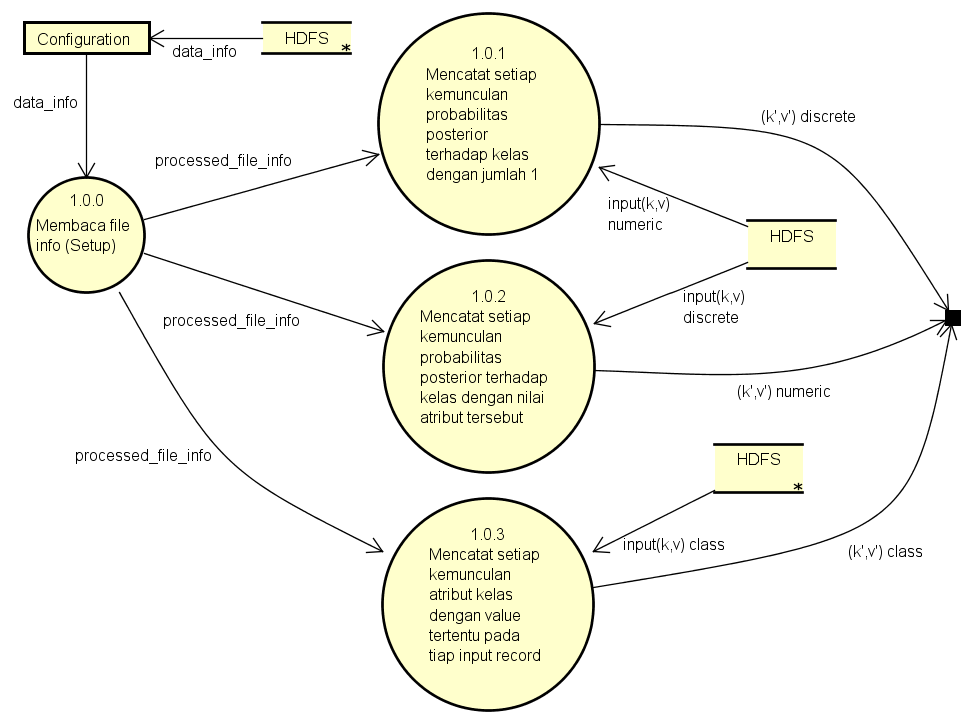
\includegraphics[scale=0.5]{Diagram/DFD_1_1_Training_Map}
	\caption[DFD level 2: proses 1.0]{DFD level 2: proses 1.0}
	\label{fig:DFD level 2: proses 1.0}
\end{figure}

\paragraph{\textit{Data Dictionary} pada DFD \textit{level} 2: proses 1.0}
\begin{enumerate}
	\item{Data \verb|data_info|}
		\begin{itemize}
			\item Nama field atribut kelas yang dipakai pada \textit{training} = [A..Z|a..z]
			\item Nama field atribut prediktor yang dipakai pada \textit{training} = [A..Z|a..z]
			\item Nomor indeks dari atribut kelas = [0..9]
			\item Nomor indeks dari atribut prediktor = [0..9]
			\item Tipe jenis atribut prediktor = [A..Z|a..z]
			\item Jumlah field yang ada pada data \textit{input} = [0..9]
		\end{itemize}
		 \textcolor{red}{*}Setiap atribut pada prediktor akan dipisahkan menggunakan karakter titik-koma\textit{(;)}.\\
	Contoh data \verb|data_info|
	\begin{lstlisting}
	<- prediktor ->
	Outlook,0,DISCRETE;Temperature,1,DISCRETE;Windy,3,DISCRETE;Rand,5,NUMERICAL
	<- kelas ->
	Play,4
	<- jumlah field ->
	6
	\end{lstlisting}
	
	\item{Data \verb|processed_file_info|}
	Isi dari data \verb|processed_file_info| sama dengan data \verb|data_info|. Tetapi, format dan jenis tipe datanya dibedakan sedikit.
	Contoh data \verb|data_info|
	\begin{lstlisting}
	<- prediktor ->
	[
		{Outlook,0,DISCRETE},
		{Temperature,1,DISCRETE},
		{Windy,3,DISCRETE},
		{Rand,5,NUMERICAL},
	]
	<- kelas ->
	[
		{Play,4},
	]
	<- jumlah field ->
	6
	\end{lstlisting}	
	
	\item{Data \verb|input(k,v)numeric|}\\
	Format pada data ini akan memiliki format sama dengan data pada \verb|data_input|. Pengecekan akan dilakukan oleh sistem yang dibuat untuk mengenali tipe atribut dari tiap field yang akan diperiksanya.	
	
	\item{Data \verb|input(k,v)discrete|}
	Format pada data ini akan memiliki format sama dengan data pada \verb|data_input|. Pengecekan akan dilakukan oleh sistem yang dibuat untuk mengenali tipe atribut dari tiap field yang akan diperiksanya.

	\item{Data \verb|(k',v')class|}
	\begin{itemize}
		\item \textit{Key} terdiri dari:
		\begin{enumerate}
			\item \textit{Class Name} = [A..Z|a..z] \textit{\textcolor{red}{*}required}
			\item \textit{Class Value} = [A..Z|a..z] \textit{\textcolor{red}{*}required}
		\end{enumerate}
		\item \textit{Value} terdiri dari:
		\begin{enumerate}
			\item Frekuensi kemunculan atribut kelas tersebut = [1](bernilai selalu 1)
		\end{enumerate}
	\end{itemize}
	
	\item{Data \verb|(k',v')discrete|}
	\begin{itemize}
		\item \textit{Key} terdiri dari:
		\begin{enumerate}
			\item \textit{Class Name} = [A..Z|a..z] \textit{\textcolor{red}{*}required}
			\item \textit{Class Value} = [A..Z|a..z] \textit{\textcolor{red}{*}required}
			\item \textit{Attribute Type} = [A..Z|a..z] \textit{\textcolor{red}{*}required}
			\item \textit{Predictor Name} = [A..Z|a..z] \textcolor{red}{*}\textit{required}
			\item \textit{Predictor Value} = [A..Z|a..z|0..9] \textcolor{red}{*}\textit{required}
		\end{enumerate}
		\item \textit{Value} terdiri dari:
		\begin{enumerate}
			\item Frekuensi kemunculan dari probabilitas posterior = [1] (bernilai selalu 1).
		\end{enumerate}
	\end{itemize}

	\item{Data \verb|(k',v')numeric|}
	\begin{itemize}
		\item \textit{Key} terdiri dari:
		\begin{enumerate}
			\item \textit{Class Name} = [A..Z|a..z] \textit{\textcolor{red}{*}required}
			\item \textit{Class Value} = [A..Z|a..z] \textit{\textcolor{red}{*}required}
			\item \textit{Attribute Type} = [A..Z|a..z] \textit{\textcolor{red}{*}required}
			\item \textit{Predictor Name} = [A..Z|a..z] \textcolor{red}{*}\textit{required}
		\end{enumerate}
		\item \textit{Value} terdiri dari:
		\begin{enumerate}
			\item Nilai dari atribut numerik tersebut = [0..9]
		\end{enumerate}
	\end{itemize}

\end{enumerate}

\paragraph{P-Spec (\textit{Process Specification}) pada DFD \textit{level} 2: pada proses 1.0}
\begin{figure}[H]
	\centering
	\includegraphics[scale=0.6]{PSpec/P-Spec_dfd_1_0_0_train}
	\caption[P-Spec proses 1.0.0]{P-Spec training map: pada proses 1.0.0}
	\label{fig:P-Spec training: pada proses 1.0.0}
\end{figure}

\begin{figure}[H]
	\centering
	\includegraphics[scale=0.6]{PSpec/P-Spec_dfd_1_0_1_train}
	\caption[P-Spec proses 1.0.1]{P-Spec training map: pada proses 1.0.1}
	\label{fig:P-Spec training: pada proses 1.0.1}
\end{figure}

\begin{figure}[H]
	\centering
	\includegraphics[scale=0.6]{PSpec/P-Spec_dfd_1_0_2_train}
	\caption[P-Spec proses 1.0.2]{P-Spec training map: pada proses 1.0.2}
	\label{fig:P-Spec training: pada proses 1.0.2}
\end{figure}

\begin{figure}[H]
	\centering
	\includegraphics[scale=0.6]{PSpec/P-Spec_dfd_1_0_3_train}
	\caption[P-Spec proses 1.0.3]{P-Spec training map: pada proses 1.0.3}
	\label{fig:P-Spec training: pada proses 1.0.3}
\end{figure}

\paragraph{DFD \textit{level} 2: pada proses 1.1}
\begin{figure}[H]
	\centering
	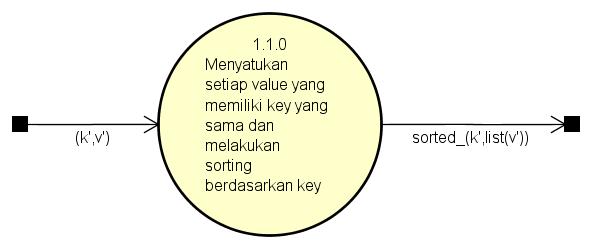
\includegraphics[scale=0.65]{Diagram/DFD_1_2_Training_Test_SS}
	\caption[DFD level 2: proses 1.1]{DFD level 2: proses 1.1}
	\label{fig:DFD level 2: proses 1.1}
\end{figure}

\paragraph{\textit{Data Dictionary} pada DFD \textit{level} 2: proses 1.1}
\begin{enumerate}
	\item{Data \verb|(k,v)|}
	\begin{itemize}
		\item \textit{Key} terdiri dari:
		\begin{enumerate}
			\item \textit{Class Name} = [A..Z|a..z] \textit{\textcolor{red}{*}required}
			\item \textit{Class Value} = [A..Z|a..z] \textit{\textcolor{red}{*}required}
			\item \textit{Attribute Type} = [A..Z|a..z] \textit{\textcolor{red}{*}required}
			\item \textit{Predictor Name} = [A..Z|a..z]
			\item \textit{Predictor Value} = [A..Z|a..z|0..9]
		\end{enumerate}
		\item \textit{Value} terdiri dari:
		\begin{enumerate}
			\item Frekuensi kemunculan dari atribut kelas = [1]
			\item Frekuensi kemunculan dari atribut prediktor = [1]
			\item Nilai dari atribut numerik = [0..9]
		\end{enumerate}
	\end{itemize}
	Contoh data \verb|(k,v)|
	\begin{lstlisting}
	key								value
	|_class|Play,Yes				1
	|cont|Rand,Play,Yes				32.5
	|disc|Humidity,High,Play,No		1
	\end{lstlisting}
	
	\item{Data \verb|sorted_(k',list(v'))|}
	Format dari variabel \textit{key} dan \textit{value} sama dengan data pada \verb|(k,v)|. Hanya tipe pada variabel \textit{value} diubah menjadi list.\\
	Contoh data \verb|sorted_(k',list(v'))|
	\begin{lstlisting}
	key								list_of_value
	|_class|Play,Yes				[1,1,1,1]
	|cont|Rand,Play,Yes				[32.5,24.5]
	|disc|Humidity,High,Play,No		[1,1]
	\end{lstlisting}
\end{enumerate}

\paragraph{P-Spec (\textit{Process Specification}) pada proses 1.1}
\begin{figure}[H]
	\centering
	\includegraphics[scale=0.6]{PSpec/P-Spec_dfd_1_1_0_train_testing}
	\caption[P-Spec training reduce: pada proses 1.1.0]{P-Spec training shuffle sort: pada proses 1.1.0}
	\label{fig:P-Spec training shuffle sort: pada proses 1.1.0}
\end{figure}


\paragraph{DFD \textit{level} 2: pada proses 1.2}
\begin{figure}[H]
	\centering
	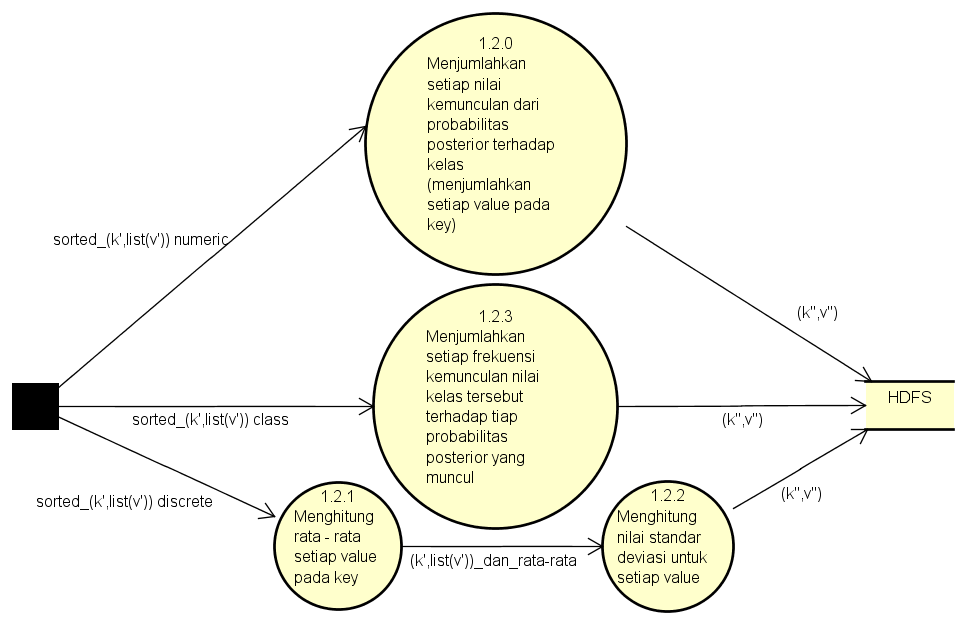
\includegraphics[scale=0.6]{Diagram/DFD_1_3_Training_Red}
	\caption[DFD level 2: proses 1.2]{DFD level 2: proses 1.2}
	\label{fig:DFD level 2: proses 1.2}
\end{figure}

\paragraph{\textit{Data Dictionary} pada DFD \textit{level} 2: proses 1.2}
\begin{enumerate}
	\item{Data \verb|sorted_(k',list(v'))numeric|}
	\begin{itemize}
		\item \textit{Key} terdiri dari:
		\begin{enumerate}
			\item \textit{Class Name} = [A..Z|a..z] \textit{\textcolor{red}{*}required}
			\item \textit{Class Value} = [A..Z|a..z] \textit{\textcolor{red}{*}required}
			\item \textit{Attribute Type} = [A..Z|a..z] \textit{\textcolor{red}{*}required}
			\item \textit{Predictor Name} = [A..Z|a..z] \textit{\textcolor{red}{*}required}
		\end{enumerate}
		\item \textit{Value} terdiri dari:
		\begin{enumerate}
			\item Nilai dari atribut numerik itu sendiri = [0..9]
		\end{enumerate}
	\end{itemize}
	Contoh data \verb|sorted_(k',list(v'))numeric|
	\begin{lstlisting}
		key							list_of_value
		|cont|Rand,Play,Yes			[32.5,25.3]
		|cont|Rand,Play,No			[40.21,54.3]
	\end{lstlisting}
	
	\item{Data \verb|sorted_(k',list(v'))discrete|}
	\begin{itemize}
		\item \textit{Key} terdiri dari:
		\begin{enumerate}
			\item \textit{Class Name} = [A..Z|a..z] \textit{\textcolor{red}{*}required}
			\item \textit{Class Value} = [A..Z|a..z] \textit{\textcolor{red}{*}required}
			\item \textit{Attribute Type} = [A..Z|a..z] \textit{\textcolor{red}{*}required}
			\item \textit{Predictor Name} = [A..Z|a..z] \textit{\textcolor{red}{*}required}
			\item \textit{Predictor Value} = [A..Z|a..z] \textit{\textcolor{red}{*}required}
		\end{enumerate}
		\item \textit{Value} terdiri dari:
		\begin{enumerate}
			\item Frekuensi kemunculan = [1]
		\end{enumerate}
	\end{itemize}
	Contoh data \verb|sorted_(k',list(v'))discrete|
	\begin{lstlisting}
		key									list_of_value
		|disc|Humidity,High,Play,No			[32.5,25.3]
		|disc|Humidity,High,Play,Yes		[40.21,54.3]
	\end{lstlisting}
	
	\item{Data \verb|sorted_(k',list(v'))class|}
	\begin{itemize}
		\item \textit{Key} terdiri dari:
		\begin{enumerate}
			\item \textit{Class Name} = [A..Z|a..z] \textit{\textcolor{red}{*}required}
			\item \textit{Class Value} = [A..Z|a..z] \textit{\textcolor{red}{*}required}
			\item \textit{Attribute Type} = [A..Z|a..z] \textit{\textcolor{red}{*}required}
		\end{enumerate}
		\item \textit{Value} terdiri dari:
		\begin{enumerate}
			\item Frekuensi kemunculan = [1]
		\end{enumerate}
	\end{itemize}
	Contoh data \verb|sorted_(k',list(v'))class|
	\begin{lstlisting}
		key						list_of_value
		|_class|Play,No			[1,1,1,1]
		|_class|Play,Yes		[1,1,1,1,1,1,1]
	\end{lstlisting}

	\item{Data \verb|sorted_(k',list(v'))_dan_rata-rata|}
	\begin{itemize}
		\item \textit{Key} terdiri dari:
		\begin{enumerate}
			\item \textit{Class Name} = [A..Z|a..z] \textit{\textcolor{red}{*}required}
			\item \textit{Class Value} = [A..Z|a..z] \textit{\textcolor{red}{*}required}
			\item \textit{Attribute Type} = [A..Z|a..z] \textit{\textcolor{red}{*}required}
		\end{enumerate}
		\item \textit{Value} terdiri dari:
		\begin{enumerate}
			\item Frekuensi kemunculan = [1]
		\end{enumerate}
		\item Rata - rata dari seluruh \textit{list of value} tersebut = [0..9]
	\end{itemize}
	Contoh data \verb|sorted_(k',list(v'))_dan_rata-rata|
	\begin{lstlisting}
		key									list_of_value	rata-rata
		|cont|Humidity,High,Play,No			[32.5,25.3]		28.9	
		|cont|Humidity,High,Play,Yes		[40.21,54.3]	47.255
	\end{lstlisting}

	\item{Data \verb|(k",v")|}
	\begin{itemize}
		\item \textit{Key} terdiri dari:
		\begin{enumerate}
			\item \textit{Class Name} = [A..Z|a..z] \textit{\textcolor{red}{*}required}
			\item \textit{Class Value} = [A..Z|a..z] \textit{\textcolor{red}{*}required}
			\item \textit{Attribute Type} = [A..Z|a..z]	\textit{\textcolor{red}{*}required}	
			\item \textit{Predictor Name} = [A..Z|a..z]	
			\item \textit{Predictor Value} = [A..Z|a..z]
			\item Frekuensi kemunculan untuk atribut diskrit/kelas = [0..9]
		\end{enumerate}
				
		\item \textit{Value} untuk atribut numerik terdiri dari:
		\begin{enumerate}
			\item \textit{Predictor Value} = [0..9] 
			\item \textit{Attribute Type} = [A..Z|a..z] 			
			\item \textit{Mean} = [0..9]
			\item \textit{Sigma} = [0..9]
		\end{enumerate}
	\end{itemize}
	Contoh data \verb|(k",v")|
	\begin{lstlisting}
	key									value
	Play,No,3.0|CLASS					(empty-string)
	Humidity,Play,Yes 					;82.5|3.5|NUMERIC
	Outlook,Sunny,Play,Yes,2.0|DISCRETE	(empty-string)
	Outlook,Rainy,Play,No,2.0|DISCRETE	(empty-string)
	\end{lstlisting}


\end{enumerate}


\paragraph{P-Spec (\textit{Process Specification}) pada proses 1.2}

\begin{figure}[H]
	\centering
	\includegraphics[scale=0.6]{PSpec/P-Spec_dfd_1_2_0_train}
	\caption[P-Spec training reduce: pada proses 1.2.0]{P-Spec training reduce: pada proses 1.2.0}
	\label{fig:P-Spec training reduce: pada proses 1.2.0}
\end{figure}

\begin{figure}[H]
	\centering
	\includegraphics[scale=0.6]{PSpec/P-Spec_dfd_1_2_1_train}
	\caption[P-Spec training reduce: pada proses 1.2.1]{P-Spec training reduce: pada proses 1.2.1}
	\label{fig:P-Spec training reduce: pada proses 1.2.1}
\end{figure}

\begin{figure}[H]
	\centering
	\includegraphics[scale=0.6]{PSpec/P-Spec_dfd_1_2_2_train}
	\caption[P-Spec training reduce: pada proses 1.2.2]{P-Spec training reduce: pada proses 1.2.2}
	\label{fig:P-Spec training reduce: pada proses 1.2.2}
\end{figure}

\begin{figure}[H]
	\centering
	\includegraphics[scale=0.6]{PSpec/P-Spec_dfd_1_2_3_train}
	\caption[P-Spec training: pada proses 1.2.3]{P-Spec training reduce: pada proses 1.2.3}
	\label{fig:P-Spec training reduce: pada proses 1.2.3}
\end{figure}


\subsubsection{Modul \textit{Testing Naive Bayes M-R Based}}

Pada modul ini, program akan memanfaatkan model klasifikasi naive bayes yang telah dibuat sebelumnya untuk melakukan klasifikasi pada data testing yang telah ada sebelumnya di HDFS (pada modul input) dan memberikan laporan analisis mengenai tingkat akurasi dan tingkat error yang dimiliki oleh model terhadap data tersebut. 

Berikut merupakan diagram \textit{flow chart} untuk modul \textit{testing}:

\begin{figure}[H]
	\centering
	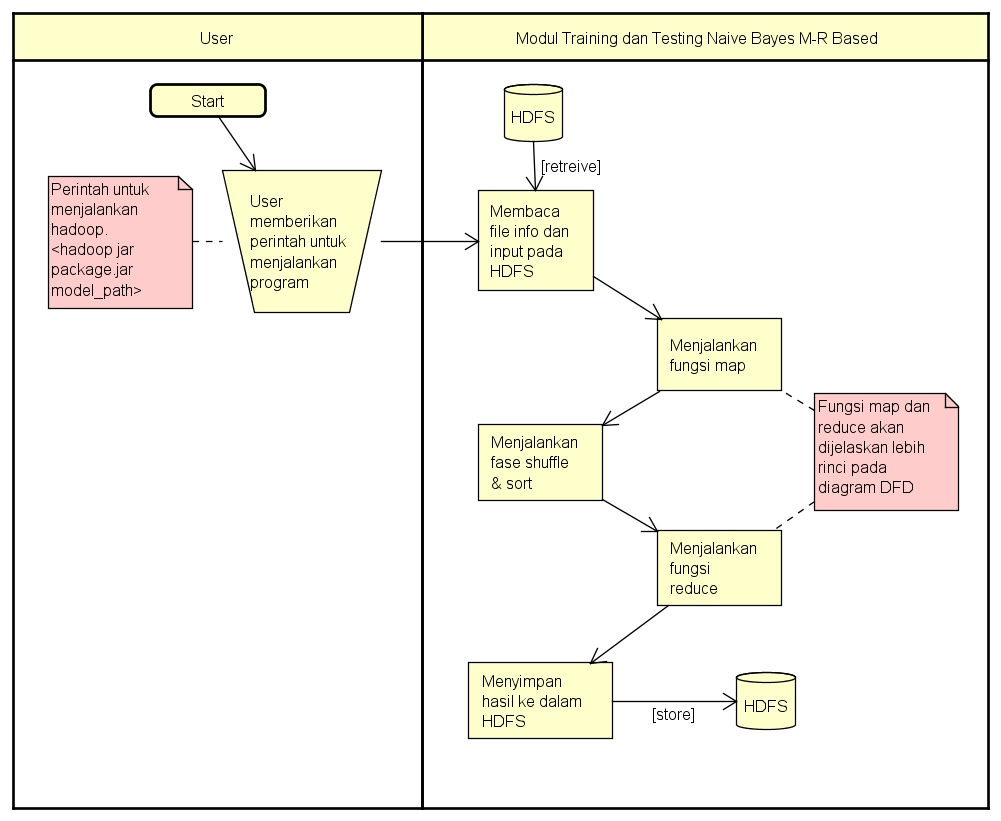
\includegraphics[scale=0.6]{Diagram/Flowchart_Training_Testing_MR}
	\caption[Flow Chart Modul Testing]{Flow Chart Modul Testing}
	\label{fig:Flow Chart Modul Testing}
\end{figure}

Sama seperti pada modul \textit{training}, untuk proses yang berbasis \textit{MapReduce} pada modul ini juga perlu digambarkan menggunakan DFD, agar bisa tergambarkan lebih rinci mengenai detail proses tersebut. Berikut merupakan \textit{context diagram}\footnote{\textit{Context Diagram biasa disebut juga sebagai DFD level 0.}} dan DFD untuk proses \textit{MapReduce} pada modul \textit{testing}:

\paragraph{\textit{Context Diagram} Modul \textit{Testing}}
\begin{figure}[H]
	\centering
	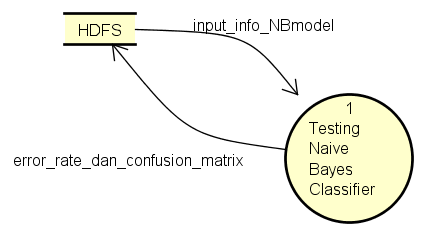
\includegraphics[scale=0.65]{Diagram/DFD_0_Testing}
	\caption[\textit{Context diagram} modul Testing]{\textit{Context diagram} modul Testing}
	\label{fig:Context diagram modul Testing}
\end{figure}

\paragraph{\textit{Data Dictionary} \textit{Context Diagram} Modul \textit{Testing}}
\begin{enumerate}
	\item{Data \verb|input_info_NBmodel|} terdiri dari input dan NBC (\textit{Naive Bayes Classifier}) model.
	\begin{itemize}
		\item \textit{Input} terdiri dari: 
		\begin{enumerate}
			\item Nilai dari atribut kelas pada input = [A..Z|a..z]
			\item Nilai dari atribut prediktor bertipe diskrit pada input = [A..Z|a..z]
			\item Nilai dari atribut prediktor bertipe numerik pada input = [0..9]
		\end{enumerate}						
		
		\item NBC model terdiri dari:
		\begin{enumerate}
			\item \textit{Class Name} = [A..Z|a..z|]
			\item \textit{Class Value} = [A..Z|a..z|] 
			\item \textit{Attribute Type} = [A..Z|a..z|] 
			\item \textit{Predictor Name} = [A..Z|a..z|]
			\item \textit{Predictor Value} = [A..Z|a..z|]
			\item Frekuensi kemunculan untuk tiap atribut kelas	= [A..Z|a..z|0..9]
			\item Frekuensi kemunculan untuk tiap atribut prediktor diskrit	= [A..Z|a..z|0..9]
			\item Nilai mean dari atribut prediktor numerik = [0..9]
			\item Nilai sigma/standard-deviasi dari atribut prediktor numerik = [0..9]
		\end{enumerate}		
		
	\end{itemize}
	Contoh data \verb|input_info_NBmodel|
	\begin{lstlisting}
	<- input ->
	Sunny,Mild,Normal,FALSE,Yes,5
	Rainy,Mild,Normal,TRUE,Yes,4.5
	Overcast,Mild,High,TRUE,Yes,3.1
	<- NBmodel ->
	Play,Yes,2.0|CLASS
	Play,No,3.0|CLASS
	Humidity,Play,Yes ;82.5|3.5|NUMERIC
	Humidity,Play,No ;71.0|9.6|NUMERIC
	Outlook,Sunny,Play,Yes,2.0|DISCRETE
	Outlook,Sunny,Play,No,1.0|DISCRETE
	Outlook,Rainy,Play,No,2.0|DISCRETE
	\end{lstlisting}
		
	\item{Data \verb|error_rate_dan_confusion_matrix|}
	\begin{itemize}
		\item Nama kelas = [A..Z|a..z]
		\item \textit{Confusion Matrix} untuk tiap kelas = matrix $n*m$
		\item \textit{Error rate} untuk $Accuracy$ untuk tiap kelas = [0..9]
		\item \textit{Error rate} untuk $Recall$ untuk tiap \textit{class value} = [0..9]
		\item \textit{Error rate} untuk $Precision$ untuk tiap \textit{class value} = [0..9]
		\item \textit{Error rate} untuk $F-Measure$ untuk tiap \textit{class value} = [0..9]
	\end{itemize}
	\begin{lstlisting}
	@play
	####
	|		|	no	| yes	|
	| no	|	3	| 0		|
	| yes	|	0	| 2		|
	####
	Accuracy: 5/5 = 1.0
	*For Value = no
	Precision: -> 3 / 3 + 0 = 1.0
	Recall: -> 3 / 3 + 0 = 1.0 
	*For Value = yes
	Precision: -> 2 / 2 + 0 = 1.0
	Recall: -> 2 / 2 + 0 = 1.0
	F-Measure -> 0.8
	\end{lstlisting}
	
\end{enumerate}


\paragraph{DFD \textit{level} 1}
\begin{figure}[H]
	\centering
	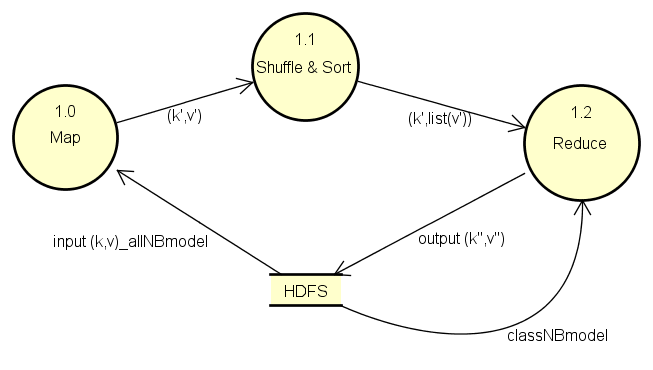
\includegraphics[scale=0.65]{Diagram/DFD_1_0_Testing_rdmodel}
	\caption[DFD level 0 modul Testing]{DFD level 0 modul Testing}
	\label{fig:DFD level 0 modul Testing}
\end{figure}

\paragraph{\textit{Data Dictionary} pada DFD \textit{level} 1}
\begin{enumerate}
	\item{Data \verb|input(k,v)_allNBmodel|}
	\begin{itemize}
		\item \textit{Key} pada \verb|input(k,v)| = \textit{NULL} (karena memang pada awal proses \textit{mapreduce} key pada input belum terdefinisi)

		\item \textit{Value} pada \verb|input(k,v)| terdiri dari:
		\begin{enumerate}
			\item Nilai tiap atribut prediktor diskrit pada input = [A..Z|a..z|]
			\item Nilai tiap atribut prediktor numerik pada input = [0..9]
			\item Nilai tiap atribut kelas pada input = [A..Z|a..z]
		\end{enumerate}

		\item \textit{allNBmodel} yang merupakan model dari NBC memiliki format sama dengan NBC model yang terdapat pada data \verb|input_info_NBmodel|.
		
	\end{itemize}
	
	\item{Data \verb|(k',v')|}
	\begin{itemize}
		\item \textit{Key} yang merupakan nama atribut kelas = [A..Z|a..z]
		\item \textit{Value} terdiri dari:
		\begin{enumerate}
			\item \textit{Class Name} = [A..Z|a..z]
			\item \textit{Class Value Predicted} = [A..Z|a..z]
			\item \textit{Class Value Actual} = [A..Z|a..z]
			\item \textit{Percentage} = [0..9]
		\end{enumerate}
	\end{itemize}
	Contoh data \verb|(k',v')|
	\begin{lstlisting}
	key			value
	Play		Play|predicted=Yes|percentage=67.5%|actual=Yes
	Play		Play|predicted=Yes|percentage=51.1%|actual=No
	Play		Play|predicted=No|percentage=96.32%|actual=No	
	\end{lstlisting}

	\item{Data \verb|(k',list(v'))|}\\
	format key dan value pada data ini sama dengan data \verb|(k',v')|. Hanya saja, untuk variabel \textit{value}-nya dijadikan sebuah list untuk setiap nama variabel \textit{key} yang sama.\\
	Contoh data \verb|(k',list(v'))|
	\begin{lstlisting}
	key			list_of_value
	Play		[
					{Play|predicted=Yes|percentage=67.5%|actual=Yes},
					{Play|predicted=Yes|percentage=51.1%|actual=No},
					{Play|predicted=No|percentage=96.32%|actual=No},
				]
	\end{lstlisting}

	\item{Data \verb|output(k",v")|}
	\begin{itemize}
		\item \textit{Key} terdiri dari:
		\begin{enumerate}
			\item \textit{Class Name} = [A..Z|a..z]
			\item \textit{Confusion Matrix} untuk tiap kelas = matrix $m*n$
		\end{enumerate}
		
		\item \textit{Value} terdiri dari:
		\begin{enumerate}
			\item \textit{Error rate} untuk $Accuracy$ untuk tiap kelas = [0..9]
			\item \textit{Error rate} untuk $Recall$ untuk tiap \textit{class value} = [0..9]
			\item \textit{Error rate} untuk $Precision$ untuk tiap \textit{class value} = [0..9]
			\item \textit{Error rate} untuk $F-Measure$ untuk tiap \textit{class value} = [0..9]
		\end{enumerate}
	\end{itemize}
	Contoh data \verb|output(k",v")|
	\begin{lstlisting}
	<- Key ->
	@play
	####
	|		|	no	| yes	|
	| no	|	3	| 0		|
	| yes	|	0	| 2		|
	####
	<- Value ->
	Accuracy: 5/5 = 1.0
	*For Value = no
	Precision: -> 3 / 3 + 0 = 1.0
	Recall: -> 3 / 3 + 0 = 1.0 
	*For Value = yes
	Precision: -> 2 / 2 + 0 = 1.0
	Recall: -> 2 / 2 + 0 = 1.0
	F-Measure -> 0.8
	\end{lstlisting}

	\item{Data \verb|classNBmodel|} yang merupakan model dari NBC memiliki format hampir sama dengan NBC model yang terdapat pada data \verb|input_info_NBmodel|. Bedanya, data ini hanya mengambil model yang bertipe atribut kelas saja untuk digunakan dalam menghitung \textit{confusion matrix}.\\
	Contoh data \verb|classNBmodel|: 
	\begin{lstlisting}
	Play,Yes,2.0|CLASS
	Play,No,3.0|CLASS
	\end{lstlisting}

\end{enumerate}


\paragraph{DFD \textit{level} 2: pada proses 1.0}
\begin{figure}[H]
	\centering
	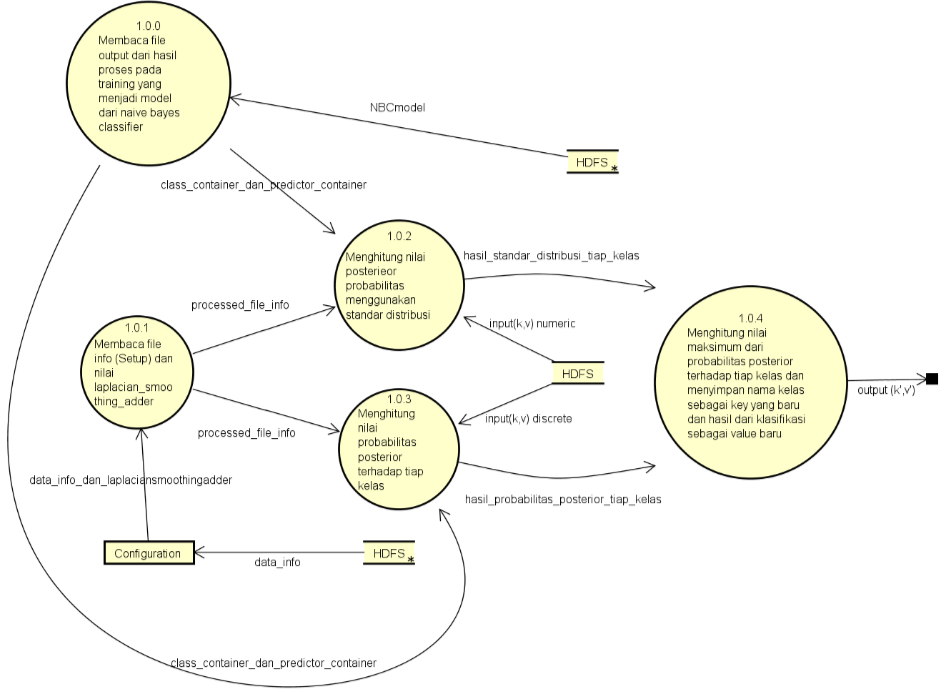
\includegraphics[scale=0.7]{Diagram/DFD_1_1_Testing_Map}
	\caption[DFD level 2: proses 1.0]{DFD level 2: proses 1.0}
	\label{fig:DFD level 2: proses 1.0}
\end{figure}

\paragraph{P-Spec (\textit{Process Specification}) pada proses 1.0}
\begin{enumerate}
	\item{Data \verb|NBCmodel|}
	yang merupakan model dari NBC memiliki format sama dengan NBC model yang terdapat pada data \verb|input_info_NBmodel| di \textit{context diagram}.
	
	\item{Data \verb|class_contanier_dan_predictor_container|}
	\begin{itemize}
		\item \textit{Class Name} = [A..Z|a..z]
		\item \textit{Class Value} = [A..Z|a..z]
		\item \textit{Predictor Name} = [A..Z|a..z]
		\item \textit{Predictor Value} = [A..Z|a..z|0..9]
		\item \textit{Attribute Type} = [A..Z|a..z]
		\item \textit{Mean} = [0..9]
		\item \textit{Sigma} = [0..9]
	\end{itemize}

	\item{Data \verb|data_info|}
	\begin{itemize}
		\item Nama tiap field = [A..Z|a..z]
		\item Nomor index tiap field = [0..9]
		\item Tipe tiap field = [A..Z|a..z]
	\end{itemize}

	\item{Data \verb|data_info_dan_laplaciansmoothingadder|} \\
	Data ini merupakan data yang sama pada data \verb|data_info|, tetapi ditambahkan nilai \textit{laplaciansmoothingadder} sebagai counter untuk penambahan tiap frekuensi probabilitas posterior untuk menghindari terjadinya permasalahan \textit{zero-frequency}.
	
	\item{Data \verb|processed_file_info|}
	Data ini merupakan data yang terdapat pada data \verb|data_info_dan_laplaciansmoothingadder|, hanya saja formatnya dibuat untuk memudahkan perangkat lunak yang nantinya dibuat membaca file info tersebut.

	\item{Data \verb|input(k,v)numeric|}
	\begin{itemize}
		\item \textit{Key} pada \verb|input(k,v)numeric| = \textit{NULL} (karena memang pada awal proses \textit{mapreduce} key pada input belum terdefinisi)

		\item \textit{Value} pada \verb|input(k,v)| terdiri dari:
		\begin{enumerate}
			\item Nilai tiap atribut prediktor numerik pada input = [0..9]
			\item Nilai tiap atribut kelas pada input = [A..Z|a..z]
		\end{enumerate}
		
	\end{itemize}

	\item{Data \verb|input(k,v)discrete|}
	\begin{itemize}
		\item \textit{Key} pada \verb|input(k,v)discrete| = \textit{NULL} (karena memang pada awal proses \textit{mapreduce} key pada input belum terdefinisi)

		\item \textit{Value} pada \verb|input(k,v)| terdiri dari:
		\begin{enumerate}
			\item Nilai tiap atribut prediktor diskrit pada input = [A..Z|a..z]
			\item Nilai tiap atribut kelas pada input = [A..Z|a..z]
		\end{enumerate}
		
	\end{itemize}

	\item{Data \verb|hasil_standar_distribusi_tiap_kelas|} merupakan nilai dari standard distribusi untuk probabilitas posterior tiap atribut numerik terhadap tiap kelas yang ada.
	\begin{itemize}
		\item \textit{Class Name} = [A..Z|a..z]
		\item \textit{Class Value} = [A..Z|a..z]
		\item \textit{Predictor Name} = [A..Z|a..z]
		\item \textit{Attribute Type} = [A..Z|a..z]
		\item Nilai standar distribusi = [0..9]
	\end{itemize}
	

	\item{Data \verb|hasil_probabilitas_posterior_tiap_kelas|}
	merupakan nilai hasil dari probabilitas posterior dari tiap atribut pada tiap atribut kelas yang ada.
	\begin{itemize}
		\item \textit{Class Name} = [A..Z|a..z]
		\item \textit{Class Value} = [A..Z|a..z]
		\item \textit{Predictor Name} = [A..Z|a..z]
		\item \textit{Predictor Value} = [A..Z|a..z]
		\item \textit{Attribute Type} = [A..Z|a..z]
		\item Hasil nilai probabilitas posterior dari tiap atribut prediktor terhadap tiap kelas = [0..9]
	\end{itemize}

	\item{Data \verb|output(k',v')|}
	\begin{itemize}
		\item \textit{Key} merupakan nama atribut kelas = [A..Z|a..z]
		
		\item \textit{Value} terdiri dari:
		\begin{enumerate}
			\item \textit{Class Name} = [A..Z|a..z]
			\item \textit{Class Value Predicted} = [A..Z|a..z]
			\item \textit{Class Actual} = [A..Z|a..z]
			\item \textit{Percentage} = [0..9]
		\end{enumerate}
		
	\end{itemize}
	Contoh data \verb|output(k',v')|:
	\begin{lstlisting}
	key			value
	Play		Play|predicted=Yes|percentage=67.5%|actual=Yes
	Play		Play|predicted=Yes|percentage=51.1%|actual=No
	Play		Play|predicted=No|percentage=96.32%|actual=No	
	\end{lstlisting}
	
\end{enumerate}


\begin{figure}[H]
	\centering
	\includegraphics[scale=0.65]{PSpec/P-Spec_dfd_1_0_9_test}
	\caption[P-Spec training reduce: pada proses 1.0.0]{P-Spec training reduce: pada proses 1.0.0}
	\label{fig:P-Spec training reduce: pada proses 1.0.0}
\end{figure}

\begin{figure}[H]
	\centering
	\includegraphics[scale=0.65]{PSpec/P-Spec_dfd_1_0_0_test}
	\caption[P-Spec training reduce: pada proses 1.0.1]{P-Spec training reduce: pada proses 1.0.1}
	\label{fig:P-Spec training reduce: pada proses 1.0.1}
\end{figure}

\begin{figure}[H]
	\centering
	\includegraphics[scale=0.65]{PSpec/P-Spec_dfd_1_0_1_test}
	\caption[P-Spec training reduce: pada proses 1.0.2]{P-Spec training reduce: pada proses 1.0.2}
	\label{fig:P-Spec training reduce: pada proses 1.0.2}
\end{figure}

\begin{figure}[H]
	\centering
	\includegraphics[scale=0.65]{PSpec/P-Spec_dfd_1_0_2_test}
	\caption[P-Spec training reduce: pada proses 1.0.3]{P-Spec training reduce: pada proses 1.0.3}
	\label{fig:P-Spec training reduce: pada proses 1.0.3}
\end{figure}

\begin{figure}[H]
	\centering
	\includegraphics[scale=0.65]{PSpec/P-Spec_dfd_1_0_3_test}
	\caption[P-Spec training reduce: pada proses 1.0.4]{P-Spec training reduce: pada proses 1.0.4}
	\label{fig:P-Spec training reduce: pada proses 1.0.4}
\end{figure}


\paragraph{DFD \textit{level} 2: pada proses 1.1}
\begin{figure}[H]
	\centering
	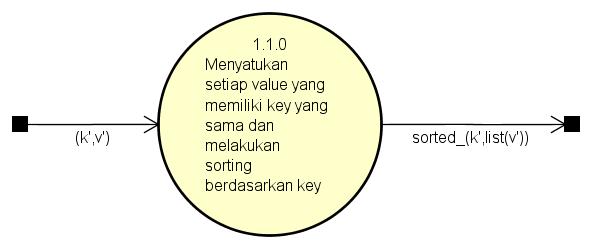
\includegraphics[scale=0.65]{Diagram/DFD_1_2_Training_Test_SS}
	\caption[DFD level 2: proses 1.1]{DFD level 2: proses 1.1}
	\label{fig:DFD level 2: proses 1.1}
\end{figure}

\paragraph{Data Dictionary pada DFD \textit{level} 2: proses 1.1}
\begin{enumerate}
	\item{Data \verb|(k',v')|} memiliki format yang sama dengan data \verb|output(k',v')| pada proses 1.0
	
	\item{Data \verb|sorted(k',list(v'))|} memiliki format yang sama dengan \textit{value} pada data \verb|output(k',v')|. Hanya saja value yang ini baru merupakan kumpulan dari \textit{value} yang memiliki \textit{key}(nama kelas) yang sama.

\end{enumerate}

\paragraph{DFD \textit{level} 2: pada proses 1.2}
\begin{figure}[H]
	\centering
	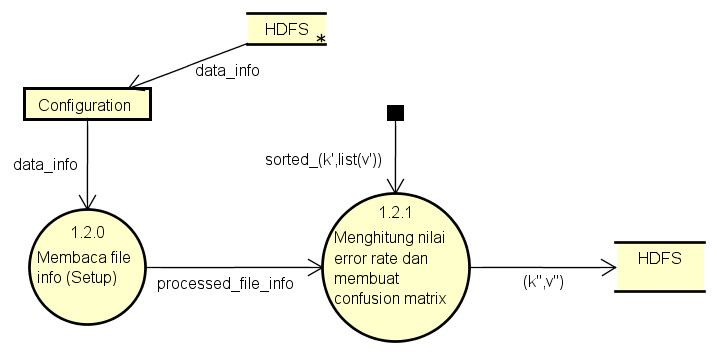
\includegraphics[scale=0.6]{Diagram/DFD_1_3_Testing_Red}
	\caption[DFD level 2: proses 1.2]{DFD level 2: proses 1.2}
	\label{fig:DFD level 2: proses 1.2}
\end{figure}

\paragraph{Data Dictionary pada DFD \textit{level} 2: proses 1.2}
\begin{enumerate}
	\item Data \verb|data_info| memiliki format dan isi yang sama dengan data \verb|data_info| pada proses 1.0
	
	\item Data \verb|processed_file_info|
	memiliki format dan isi yang mirip dengan data \verb|processed_file_info| pada proses 1.0. Hanya saja tidak mengikutsertakan nilai \textit{laplaciansmoothingadder}.

	\item Data \verb|sorted_(k',list(v'))|
	memiliki format dan isi yang sama dengan data \verb|sorted_(k',list(v'))| pada proses 1.1.

	\item Data \verb|(k",v")|
	\begin{enumerate}
		\item \textit{Key} terdiri dari:
		\begin{itemize}
			\item \textit{Class Name} = [A..Z|a..z]
			\item \textit{Confusion Matrix} = matrix $n*m$
		\end{itemize}

		\item \textit{Value} terdiri dari:
		\begin{itemize}
			\item \textit{Confusion Matrix} untuk tiap kelas = matrix $n*m$
			\item \textit{Error rate} untuk $Accuracy$ untuk tiap kelas = [0..9]
			\item \textit{Error rate} untuk $Recall$ untuk tiap \textit{class value} = [0..9]
			\item \textit{Error rate} untuk $Precision$ untuk tiap \textit{class value} = [0..9]
			\item \textit{Error rate} untuk $F-Measure$ untuk tiap \textit{class value} = [0..9]
		\end{itemize}
		Contoh data \verb|output(k",v")|
		\begin{lstlisting}
		<- Key ->
		@play
		####
		|		|	no	| yes	|
		| no	|	3	| 0		|
		| yes	|	0	| 2		|
		####
		<- Value ->
		Accuracy: 5/5 = 1.0
		*For Value = no
		Precision: -> 3 / 3 + 0 = 1.0
		Recall: -> 3 / 3 + 0 = 1.0 
		*For Value = yes
		Precision: -> 2 / 2 + 0 = 1.0
		Recall: -> 2 / 2 + 0 = 1.0
		F-Measure -> 0.8
		\end{lstlisting}
	\end{enumerate}

\end{enumerate}

\paragraph{P-Spec (\textit{Process Specification}) pada proses 1.0}

\begin{figure}[H]
	\centering
	\includegraphics[scale=0.65]{PSpec/P-Spec_dfd_1_2_0_test}
	\caption[P-Spec testing reduce: pada proses 1.2.0]{P-Spec testing reduce: pada proses 1.2.0}
	\label{fig:P-Spec testing reduce: pada proses 1.2.0}
\end{figure}

\begin{figure}[H]
	\centering
	\includegraphics[scale=0.65]{PSpec/P-Spec_dfd_1_2_1_test}
	\caption[P-Spec testing reduce: pada proses 1.2.1]{P-Spec testing reduce: pada proses 1.2.1}
	\label{fig:P-Spec testing reduce: pada proses 1.2.1}
\end{figure}


\subsubsection{Modul Klasifikasi \textit{Naive Bayes}}

Pada modul ini, program juga akan memanfaatkan model klasifikasi naive bayes yang telah dibuat sebelumnya untuk melakukan klasifikasi. Program pada modul ini dapat menerima 1 jenis input yang merupakan input manual secara satu - persatu atribut yang diperlukan untuk melakukan klasifikasi (\textit{predict new case}).

Berikut merupakan diagram \textit{flow chart} untuk modul klasifikasi:

\begin{figure}[H]
	\centering
	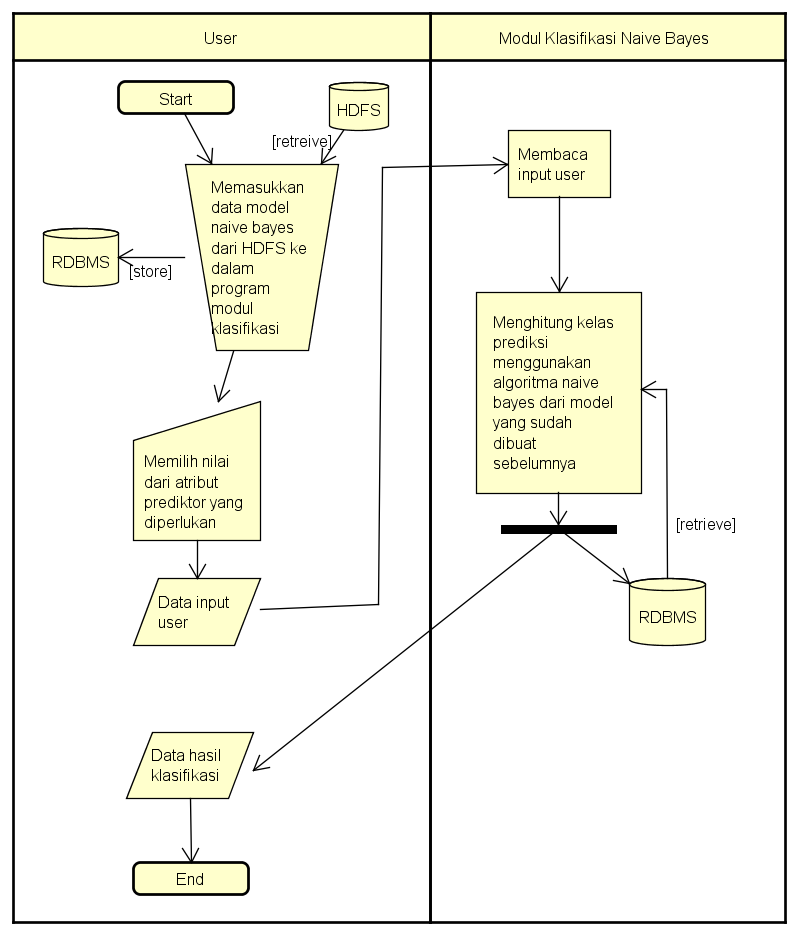
\includegraphics[scale=0.65]{Diagram/Flowchart_Klasifikasi}
	\caption[Flow Chart Modul Klasifikasi]{Flow Chart Modul Klasifikasi}
	\label{fig:Flow Chart Modul Klasifikasi}
\end{figure}

\subsection{Diagram Kelas}

Perangkat lunak yang dibangun akan mengikuti metode pemrograman berbasis objek (\textit{Object Oriented Programming}). Sehingga, untuk melakukan pemodelan pada perangkat lunak yang dibuat akan menggunakan kelas yang memiliki beberapa atribut dan metode operasi. Berikut merupakan gambaran diagram kelas pada perangkat lunak untuk setiap modul.

\subsubsection{Modul Kelola \textit{Input}}

\begin{figure}[H]
	\centering
	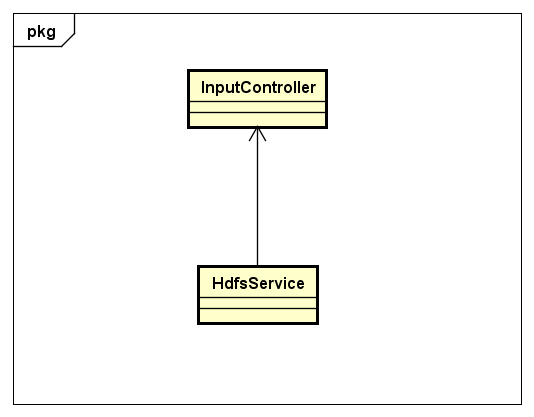
\includegraphics[scale=0.7]{ClassDiagram/Simple_CD_Input}
	\caption[Diagram kelas modul kelola input]{Diagram kelas modul kelola input}
	\label{fig:Diagram kelas modul kelola input}
\end{figure}

Pada modul ini, akan dibuatkan 2 kelas utama untuk menangani proses memasukkan file input ke dalam HDFS. Kelas tersebut diantaranya adalah:
\begin{enumerate}
\item{\textit{InputController.class}} \\
Kelas ini akan menjadi sebagai kelas yang meng-enkapsulasi seluruh proses penting yang dibutuhkan untuk memasukan file input ke dalam HDFS. Kelas ini hanya membuatkan satu method untuk melakukan operasi input yang akan diakses oleh user. Kelas ini akan memiliki objek instansiasi dari kelas \textit{HdfsService.class} dan memanggil beberapa method di dalamnya untuk melakukan operasi penulisan ke dalam HDFS.
\item{HdfsService.class} \\
Kelas ini akan mengatur segala kebutuhan yang diperlukan untuk melakukan proses penulisan ke dalam HDFS. Kelas ini akan memiliki koneksi terhadap HDFS Master sebagai \textit{hadoop client} untuk memerintahkan penulisan dan pendistribusian file baru yang akan dimasukkan ke dalam HDFS.
\end{enumerate}

\subsubsection{Modul \textit{Training dan Testing Naive Bayes M-R Based}}

\begin{figure}[H]
	\centering
	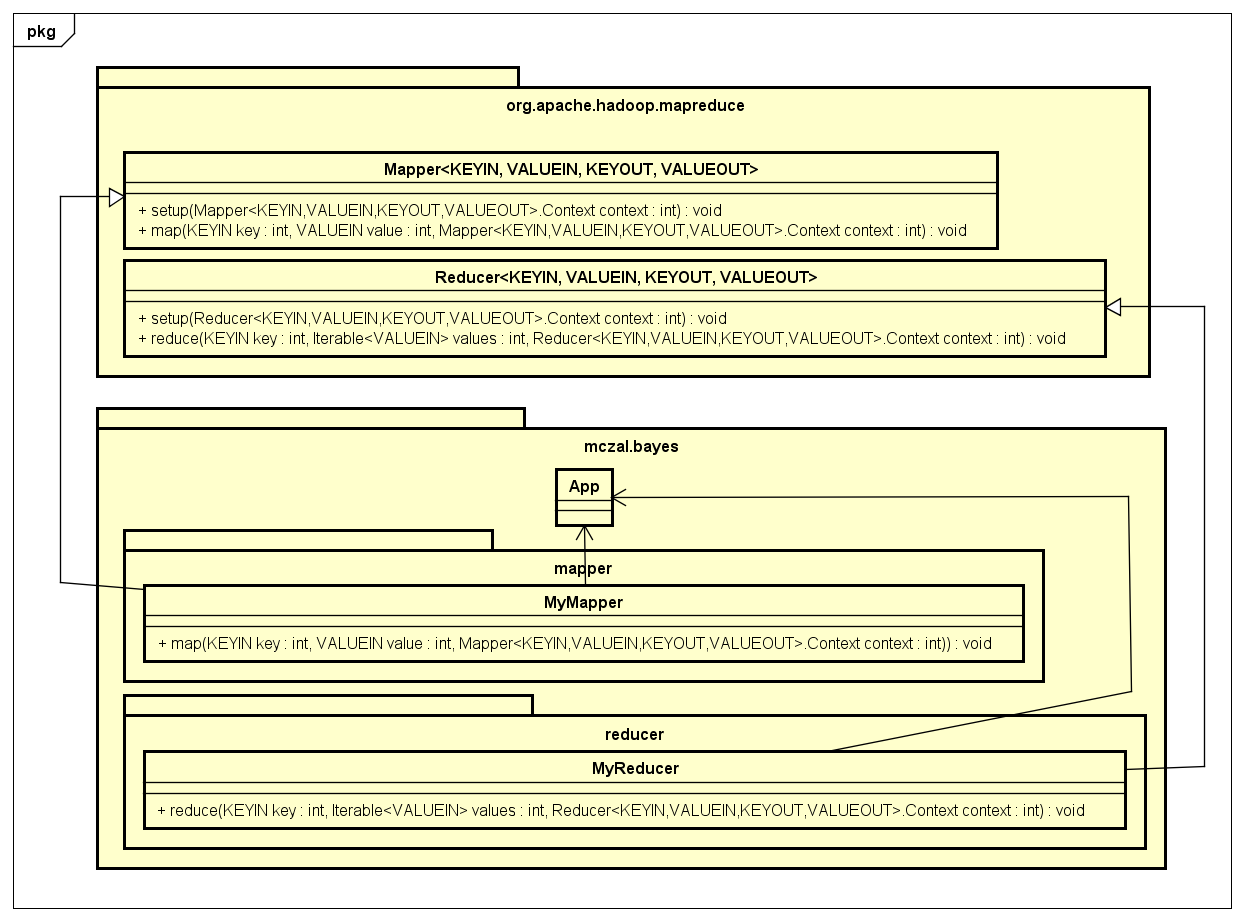
\includegraphics[scale=0.54]{ClassDiagram/Class_Diagram_Train_Test_MR}
	\caption[Diagram kelas modul \textit{training} dan \textit{testing}]{Diagram kelas modul \textit{training} dan \textit{testing}}
	\label{fig:Diagram kelas modul training dan testing}
\end{figure}

Pada modul ini, akan dibuatkan 3 kelas utama untuk menangani proses \textit{training} dan \textit{testing} berbasis \textit{MapReduce}. Kelas tersebut diantaranya adalah: 

\begin{enumerate}
\item{App.class} \\
Kelas ini akan menjadi kelas utama yang akan menjalankan operasi \textit{testing} maupun \textit{training} yang berbasis \textit{MapReduce}. Pada kelas ini akan ditentukan pula kelas mana saja yang akan dijadikan sebagai kelas mapper dan kelas reducer nya, begitu juga dengan pasangan \textit{key} dan \textit{value} untuk \textit{input} dan untuk \textit{output} di setiap kelas.
\item{MyMapper.class} \\
Kelas ini akan menjalankan operasi pada fase map untuk proses training dan testing berbasis \textit{MapReduce}.
\item{MyReducer.class} \\
Kelas ini akan menjalankan operasi pada fase reduce untuk proses training dan testing berbasis \textit{MapReduce}.
\end{enumerate}

\subsubsection{Modul Klasifikasi \textit{Naive Bayes}}
\begin{figure}[H]
	\centering
	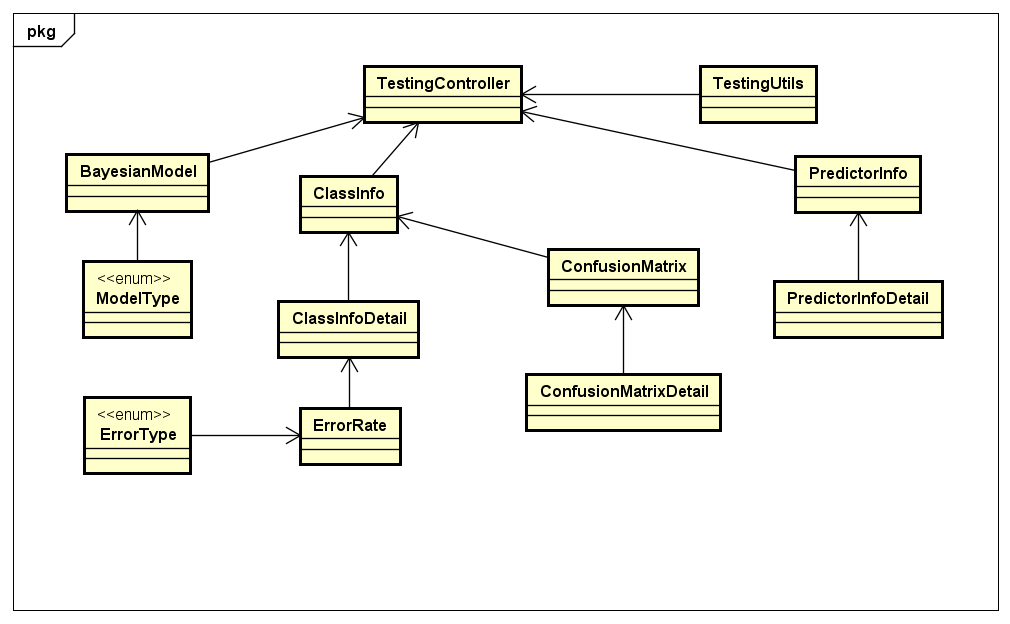
\includegraphics[scale=0.65]{ClassDiagram/Simple_CD_Klasifikasi}
	\caption[Diagram kelas modul klasifikasi \textit{naive bayes}]{Diagram kelas modul klasifikasi \textit{naive bayes}}
	\label{fig:Diagram kelas modul klasifikasi naive bayes}
\end{figure}

Pada modul ini, akan dibuatkan 10 kelas utama dan 2 kelas yang bertipe emum untuk menangani proses klasifikasi menggunakan model yang telah dibuat sebelumnya. Kelas tersebut diantaranya adalah: 
\begin{enumerate}
\item{\textit{TestingController.class}} \\
Kelas ini merupakan kelas utama yang akan melakukan enkapsulasi seluruh proses penting yang akan dijalankan pada proses klasifikasi.
\item{\textit{TestingUtils.class}} \\
Kelas ini akan menjadi kelas-pembantu pada kelas \textit{TestingController.class} untuk melakukan operasi - operasi yang dibutuhkan pada algoritma klasifikasi \textit{naive bayes}. Seperti perhitungan probabilitas posterior dan normal distribusi
\item{\textit{BayesianModel.class}} \\
Kelas ini merupakan kelas utama untuk merepresentasikan model klasifikasi \textit{naive bayes} yang telah dibuat sebelumnya.
\item{\textit{ModelType.enum}} \\
Enum ini akan menjadi tipe untuk setiap model yang ada pada kelas \textit{BayesianModel}. Enum tersebut terdiri antara: DISCRETE, NUMERIC, dan CLASS.
\item{\textit{ClassInfo.class}} \\
Kelas ini akan merepresentasikan seluruh atribut kelas pada model klasifikasi \textit{naive bayes} yang telah dibuat sebelumnya.
\item{\textit{ClassInfoDetail.class}} \\
Kelas ini merupakan ekstensi dari kelas \textit{ClassInfo.class}. Kelas ini akan menyimpan seluruh detail mengenai atribut kelas tertentu pada model \textit{naive bayes} yang sudah jadi.
\item{\textit{ErrorRate.class}} \\
Kelas ini akan merepresentasikan perhitungan \textit{ErrorRate} yang dapat dihitung setelah melakukan testing terhadap model \textit{naive bayes} yang sudah jadi sebelumnya.
\item{\textit{ErrorType.enum}} \\
Enum ini akan menjadi tipe untuk tiap error yang ada. Enum tersebut terdiri dari: $ACCURACY$, $PRECISION$, $RECALL$, dan $F_MEASURE$.
\item{\textit{ConfusionMatrix.class}} \\
Kelas ini akan merepresentasikan \textit{ConfusionMatrix} yang akan diperoleh setelah menjalani testing/klasifikasi pada model \textit{naive bayes} yang sudah jadi sebelumnya.
\item{\textit{ConfusionMatrixDetail.class}} \\
Kelas ini merupakan ekstensi dari kelas \textit{ConfusionMatrix.class}. Kelas ini akan menyimpan seluruh detail yang dimiliki oleh tiap instansiasi dari kelas \textit{ConfusionMatrix}.
\item{\textit{PredictorInfo.class}} \\
Kelas ini akan merepresentasikan sebagai seluruh atribut prediktor yang digunakan pada model \textit{naive bayes}.
\item{\textit{PredictorInfoDetail.class}} \\
Kelas ini merupakan kelas ekstensi dari kelas \textit{PredictorInfo.class}. Kelas ini akan menyimpan seluruh detail pad tiap instansiasi dari kelas \textit{PredictorInfo}.
\end{enumerate}

